%%%%%%%% ICML 2025 EXAMPLE LATEX SUBMISSION FILE %%%%%%%%%%%%%%%%%

\documentclass{article}

% Recommended, but optional, packages for figures and better typesetting:
% \usepackage{algpseudocode}
\usepackage{threeparttable}
\usepackage{microtype}
\usepackage{graphicx}
\usepackage{subcaption}
% \usepackage[inline]{showlabels}
\usepackage{booktabs} % for professional tables
% hyperref makes hyperlinks in the resulting PDF.
% If your build breaks (sometimes temporarily if a hyperlink spans a page)
% please comment out the following usepackage line and replace
% \usepackage{icml2025} with \usepackage[nohyperref]{icml2025} above.
\usepackage{hyperref}


% Attempt to make hyperref and algorithmic work together better:
\newcommand{\theHalgorithm}{\arabic{algorithm}}

% Use the following line for the initial blind version submitted for review:
% \usepackage{icml2025}

% If accepted, instead use the following line for the camera-ready submission:
\usepackage[accepted]{icml2025}

% For theorems and such
\usepackage{amsmath}
\usepackage{amssymb}
\usepackage{mathtools}
\usepackage{amsthm}
\usepackage{enumitem}

% if you use cleveref..
\usepackage[capitalize,noabbrev]{cleveref}

%%%%%%%%%%%%%%%%%%%%%%%%%%%%%%%%
% THEOREMS
%%%%%%%%%%%%%%%%%%%%%%%%%%%%%%%%
\theoremstyle{plain}
\newtheorem{theorem}{Theorem}[section]
\newtheorem{proposition}[theorem]{Proposition}
\newtheorem{lemma}[theorem]{Lemma}
\newtheorem{corollary}[theorem]{Corollary}
\theoremstyle{definition}
\newtheorem{definition}[theorem]{Definition}
\newtheorem{assumption}[theorem]{Assumption}
\theoremstyle{remark}
\newtheorem{remark}[theorem]{Remark}


\newcommand{\utr}{\texttt{UTR}}
\newcommand{\atr}{\texttt{ATR}}
\newcommand{\arc}{\texttt{CubicReg}}
\newcommand{\arca}{\texttt{CubicReg-A}}
\definecolor{rr}{RGB}{190,88,69}
\newcommand{\cz}[1]{{\color{rr} #1}}
\setlist[itemize]{leftmargin=*,label=$\bullet$,topsep=2pt,itemsep=0pt}
\setlist[enumerate]{label=$(\arabic*)$, leftmargin=*,topsep=2pt,itemsep=0pt}
% Todonotes is useful during development; simply uncomment the next line
%    and comment out the line below the next line to turn off comments
%\usepackage[disable,textsize=tiny]{todonotes}
\usepackage[textsize=tiny]{todonotes}


% The \icmltitle you define below is probably too long as a header.
% Therefore, a short form for the running title is supplied here:
\icmltitlerunning{Submission and Formatting Instructions for ICML 2025}

\begin{document}

\twocolumn[
    \icmltitle{Towards Faster Trust-Region-Type Methods: Acceleration with Constrained Subproblems}

    % It is OKAY to include author information, even for blind
    % submissions: the style file will automatically remove it for you
    % unless you've provided the [accepted] option to the icml2025
    % package.

    % List of affiliations: The first argument should be a (short)
    % identifier you will use later to specify author affiliations
    % Academic affiliations should list Department, University, City, Region, Country
    % Industry affiliations should list Company, City, Region, Country

    % You can specify symbols, otherwise they are numbered in order.
    % Ideally, you should not use this facility. Affiliations will be numbered
    % in order of appearance and this is the preferred way.
    \icmlsetsymbol{equal}{*}

    \begin{icmlauthorlist}
        \icmlauthor{Yuntian Jiang}{yyy}
        \icmlauthor{Chuwen Zhang}{yyy}
        \icmlauthor{Bo Jiang}{yyy}
        \icmlauthor{Yinyu Ye}{xxx}
        %\icmlauthor{}{sch}
        %\icmlauthor{}{sch}
    \end{icmlauthorlist}

    \icmlaffiliation{yyy}{Research Institute for Interdisciplinary Sciences, Shanghai University of Finance and Economics, Shanghai, China}
    \icmlaffiliation{xxx}{Department of Management Science and Engineering, Stanford University, CA, United States}


    \icmlcorrespondingauthor{Chuwen Zhang}{chuwzhang@gmail.com}
    \icmlcorrespondingauthor{Bo Jiang}{isyebojiang@gmail.com}

    % You may provide any keywords that you
    % find helpful for describing your paper; these are used to populate
    % the "keywords" metadata in the PDF but will not be shown in the document
    \icmlkeywords{Machine Learning, ICML}

    \vskip 0.3in
]

% this must go after the closing bracket ] following \twocolumn[ ...

% This command actually creates the footnote in the first column
% listing the affiliations and the copyright notice.
% The command takes one argument, which is text to display at the start of the footnote.
% The \icmlEqualContribution command is standard text for equal contribution.
% Remove it (just {}) if you do not need this facility.

\printAffiliationsAndNotice{}  % leave blank if no need to mention equal contribution
% \printAffiliationsAndNotice{\icmlEqualContribution} % otherwise use the standard text.

\begin{abstract}
    % Trust-region-type methods are fundamental schemes in optimization due to their excellent practical performance. However, the ball-constrained subproblems pose significant obstacles to complexity analysis, making it a daunting task to devise acceleration schemes. Building on this longstanding challenge, we propose a novel algorithmic framework for trust-region-type methods, capturing their essential characteristics to enable acceleration through refined analytical techniques. This leads to the development of the first accelerated trust-region-type algorithm with an improved global iteration complexity of $O(\epsilon^{-1/3})$. Numerical experiments demonstrate that the proposed algorithm achieves performance comparable to Nesterov's accelerated cubic Newton method, while consistently outperforming non-accelerated trust-region-type methods and the cubic Newton method.
    \cz{
        Trust-region-type methods are fundamental schemes in optimization due to their excellent practical performance. However, the ball-constrained subproblems pose significant obstacles to complexity analysis in convex settings, making it a daunting task to devise acceleration schemes. In this paper, we capture the fundamental characteristics of the trust-region subproblem and use a new analysis to make the estimating sequence technique compatible with the trust-region subproblem. This leads to the development of the \emph{first} accelerated trust-region algorithm with an improved global iteration complexity of $O(\epsilon^{-1/3})$. Numerical experiments demonstrate that the proposed algorithm achieves performance comparable to Nesterov's accelerated cubic Newton method, while consistently outperforming non-accelerated trust-region-type methods and the cubic Newton method.
    }
\end{abstract}

\section{Introduction}
\label{Intro}
The trust-region (TR) method \cite{More1983,conn2000trust} is recognized as a powerful second-order method due to its effectiveness in solving practical problems and its significant impact across various fields. It has been successfully applied in machine learning applications, such as adversarial neural networks \cite{yao2019trust}, real-time tracking \cite{liu2004real}, and mixed norm regression \cite{kim2010scalable}. Notably, the trust-region method has also inspired the widely used trust-region policy optimization \cite{schulman2015trust, kurutach2018model} in the reinforcement learning community.

In this paper, we consider the unconstrained optimization problem \begin{equation} \label{eq.main problem} \min_{x\in \mathbb{R}^n}~ f(x), \end{equation} where $f:\mathbb{R}^n\to \mathbb{R}$ satisfies Assumption~\ref{assm.solvable}-\ref{assm.bounded hessian}. The standard trust-region method operates on the local quadratic approximation of the objective function at point $x\in\mathbb{R}^n$ within a trust-region ball:
\begin{equation}
    \label{eq.classic tr subproblem} \begin{aligned} \min_{d \in \mathbb{R}^n} \  & m^{\text{TR}}(d):= \nabla f(x)^T d+\frac{1}{2}d^T \nabla^2 f(x) d, \\ \operatorname{s.t.} \ &\|d\|\le \Delta.
    \end{aligned}
\end{equation}
The solution to this subproblem is distinguished by the step $d$ and the multiplier $\lambda$ to the ball constraint.

While it has been the cornerstone for nonlinear programming and demonstrated outstanding success in practice \cite{byrdKnitroIntegratedPackage2006a}, its theoretical underpinnings are still evolving, and complexity analyses have proven challenging.

Historically, the convergence analyses of the standard trust-region method were primarily asymptotic, offering little insight into global complexity. Foundational results can be found in the textbook~\cite{conn2000trust} and the review~\cite{yuan2015recent}.

Recently, global complexity has emerged as a crucial metric for evaluating optimization algorithms. Early studies established that the standard trust-region method \cite{nocedal1999numerical,conn2000trust,cartisComplexitySteepestDescent2010,cartisComplexityBoundsSecondorder2012} converges to stationary points with an iteration complexity of $O(\epsilon^{-2})$, being suboptimal in terms of second-order methods \cz{\cite{carmon2021lower}}. Various new variants of trust-region methods are proposed to achieve global iteration complexity of $O(\epsilon^{-3/2})$. For example, see~\citet{luenberger_linear_2021, curtis2017trust, curtis2021trust, hamad2022consistently, hamad2024simplepracticaladaptivetrustregion}, albeit with different algorithmic design and analytical techniques. For details on their approaches, we refer readers to their respective works. For convex optimization, \citet{jiang2024nonconvexityuniversaltrustregionmethod} proposed a universal trust-region method with an iteration complexity of $O(\epsilon^{-1/2})$ very recently.

\cz{
    We acknowledge the significant contributions of the above results; however, there remains considerable room for trust-region methods to improve. In convex optimization, acceleration techniques~\cite{nesterovMethodSolvingConvex1983a,nesterov_lectures_2018} have emerged as a critical aspect of the research, due to theoretical and practical successes of accelerated first-order methods in machine learning~\cite{lan_first-order_2020,lin2020accelerated}.
}

This growing interest extends to accelerating the second-order methods. \citet{nesterov2008accelerating} showed that it is possible to accelerate the cubic regularized Newton method~\cite{nesterov2006cubic}, which relies on a different \emph{unconstrained} cubic-regularized subproblem of the following form at point $x$:
\begin{equation}
    \label{eq.cr update}
    \min_{d \in \mathbb{R}^n} \  m^{\text{CR}}(d):=\nabla f(x)^T d+\frac{1}{2}d^T \nabla^2 f(x) d+\frac{M}{6}\|d\|^3,
\end{equation}
where $M>0$ is defined in Assumption~\ref{assm.main assm}. This method holds significant promise due to its ability to handle convex problems. Specifically, its iteration complexity can be further accelerated to $O(\epsilon^{-1/3})$ from $O(\epsilon^{-1/2})$ for convex problems. This marks a stark contrast to the current limitations of trust-region-type methods.

Beyond cubic regularization, other accelerated second-order approaches have been developed~\cite{monteiro2013accelerated,carmon2022optimal,doikov2020contracting}. However, all the above methods stick with \emph{unconstrained subproblems} and thus can avoid the sophisticated discussion over the multiplier. However, trust-region-type methods remain obviously absent from this landscape in the presence of the ball constraint of trust-region subproblems, where suitable treatment for the \emph{dual multiplier} $\lambda$ is required.

\cz{
    Building on these observations, an essential question arises for advancing the theoretical understanding of trust-region-type methods in convex optimization:
    \begin{center}
        \emph{How to deal with the constraint in the trust-region-type method to achieve an acceleration?}
    \end{center}
}

To illustrate the difficulty, we begin by revisiting a key property required for acceleration, referred to as the \emph{regularity condition} (Definition~\ref{def.regularity condition}).

The regularity condition plays a crucial role in enabling the estimating sequence technique \cite{baesEstimateSequenceMethods2009a,nesterov_lectures_2018}, which serves as a key tool for accelerating algorithms. This technique relies on establishing a recursive relationship involving the function value across iterations, ensuring consistent cumulative progress that ultimately leads to acceleration. The cumulative progress in function value is naturally ensured by the regularity condition, which is specifically designed to support this kind of iterative setting.

Accelerated algorithms, such as the accelerated cubic regularized Newton method \cite{nesterov2008accelerating}, rely on unconstrained regularized subproblems and benefit from the key feature that the regularizer of the update is naturally proportional to the step size. This property ensures that the regularity condition holds for the update, allowing the algorithm to be directly accelerated by the estimating sequence technique.

In contrast, trust-region-type subproblems introduce posterior multipliers, creating complex dependencies between the step size and the regularizer, which is influenced by the posterior multiplier $\lambda$ \cite{nocedal1999numerical,cartis2022evaluation}. Consequently, trust-region methods do not consistently satisfy the regularity condition, failing to guarantee the function value decrease required for acceleration by the estimating sequence technique.
\paragraph{Our approach}
To address the challenge of the incompatibility between trust-region methods and the estimating sequence technique, we adopt and modify the trust-region subproblem introduced by~\citet{jiang2024nonconvexityuniversaltrustregionmethod} and design an acceleration scheme tailored for trust-region-type methods, which adjusts the way of updating based on the feedback of the multiplier.

Technically, we carefully examine the fundamental differences in iteration mechanisms between trust-region-type methods and other second-order algorithms, focusing on their distinctive feature of making progress through either reducing the function value or decreasing the gradient norm. Building on this observation, we design a customized acceleration framework (Algorithm~\ref{alg.accelerated utr}) that effectively integrates these two complementary modes of progress. Specifically, when the function value decreases sufficiently, we bypass the verification of the regularity condition and directly proceed with the update. In cases where the gradient norm contracts, we incorporate the local detection subroutine (Algorithm~\ref{alg.rr}) into the framework, ensuring that either an approximate solution or a step satisfying the regularity condition is obtained.
\begin{table*}[t]
    \caption{A Summary of the Mainstream Second-Order Methods}
    \label{table.summary}
    \vskip 0.15in
    \begin{center}
        \begin{small}
            \begin{sc}
                \begin{tabular}{lcccr}
                    \toprule
                    Alg. Type         & Nonconvex                 & Convex                                                  & Acceleration                     \\
                    \midrule
                    Cubic Newton      & \citet{nesterov2006cubic} & \citet{nesterov2006cubic}                               & \citet{nesterov2008accelerating} \\
                    Grad. Reg. Newton & \citet{gratton2023yet}    & \citet{mishchenko_regularized_2023}                     & \citet{doikov2020contracting}    \\
                    Trust-Region      & $\dagger$                 & \citet{jiang2024nonconvexityuniversaltrustregionmethod} & This Paper                       \\
                    \bottomrule
                \end{tabular}
            \end{sc}
        \end{small}
    \end{center}
    \vskip -0.1in
    \begin{tablenotes}
        \small
        \item $\dagger$ denotes the works~\cite{curtis2017trust,curtis2021trust,luenberger_linear_2021,hamad2022consistently,hamad2024simplepracticaladaptivetrustregion}.
    \end{tablenotes}
\end{table*}
\paragraph{Contribution}
In this paper, we apply the estimating sequence technique for the first time to accelerate trust-region type algorithms, which involve a constrained subproblem that needs special handling. In particular, we design the first accelerated trust-region-type method that achieves a global iteration complexity of $O(\epsilon^{-1/3})$ for finding $\epsilon$-approximate solutions in convex optimization. We remark that the number of subproblems we solve in each iteration scales logarithmically with the desired accuracy, resulting in a total complexity of $\tilde{O}(\epsilon^{-1/3})$. Notably, the subproblems within the same iteration share a similar structure, minimizing the additional computational burden.

Numerical experiments demonstrate the efficacy of our method. It is comparable to the accelerated cubic Newton method~\cite{nesterov2008accelerating} and outperforms the non-accelerated counterparts of both the trust-region method for convex optimization~\cite{jiang2024nonconvexityuniversaltrustregionmethod} and the accelerated cubic Newton method~\cite{nesterov2006cubic}.
\paragraph{Related Works}
We now provide a literature review, with a focus on further discussing the accelerated second-order algorithms mentioned earlier. Apart from the accelerated cubic Newton method, another significant development in the accelerated second-order method is the MS acceleration framework proposed by~\cite{monteiro2013accelerated} and further developed by~\citet{NEURIPS2022_e56f394b,carmon2022optimal}, which serves as a general approach for incorporating second-order methods as inner oracles, achieving an iteration complexity of $O(\epsilon^{-2/7})$. \citet{carmon2022optimal} further demonstrated that some second-order methods qualify as oracles within the MS framework.

More recently, a new second-order method employing gradient regularization was introduced by~\citet{mishchenko_regularized_2023}. This approach can be accelerated using the contracting mapping technique~\cite{doikov2020contracting}, leading to the development of the accelerated gradient regularized Newton method, which achieves a global iteration complexity of $O(\epsilon^{-1/3})$. In each iteration, they also solve a number of subproblems whose quantity scales logarithmically with the desired accuracy, but unlike ours, these subproblems lack a common structure.

\cz{
    To the best of our knowledge, the work \cite{carmon2018accelerated} is the only one that addresses accelerating algorithms with a constrained subproblem. Their method employs a subproblem that includes a ball constraint with a fixed radius $r > 0$ at $x$:
    \begin{equation}
        \label{eq.ball oracle}
        \begin{aligned} \min_{d \in \mathbb{R}^n} \ &f(x+d), \\ \operatorname{s.t.} \ &\|d\|\le r. \end{aligned}
    \end{equation}
    They focus on the complexity of approximately solving problem~\eqref{eq.main problem} with respect to the radius $r > 0$ and achieve an acceleration, improving the complexity from $\tilde O\left(R/r\right)$ to $\tilde O\left(\left(R/r\right)^{2/3}\right)$, where $R := \|x_0 - x^*\|$. They also provide a trust-region-type solver to approximately solve their subproblem~\eqref{eq.ball oracle}, which relies on a stable Hessian assumption. The differing assumptions and complexity measures lead to significant differences in how the constraint is handled and how the complexity is analyzed. Interested readers are referred to their paper for further details.
}

We conclude the convergence behavior of the aforementioned mainstream second-order methods in Table~\ref{table.summary}. We remark that the results within rely on different assumptions, please refer to their paper for details.




\section{Preliminaries}
\label{priliminary}
Let $\|\cdot\|$ denote the standard Euclidean norm in $\mathbb{R}^n$, and let $x^T y$ and $\langle x,y\rangle$ represent the inner product between $x, y \in \mathbb{R}^n$. For a matrix $A \in \mathbb{R}^{n \times n}$, $\|A\|$ denotes the induced $\ell_2$ norm. We use the standard asymptotic notations $O(\cdot), \Omega(\cdot), \Theta(\cdot)$ in their conventional sense, where $\tilde{O}(\cdot)$ hides logarithmic terms within $O(\cdot)$. Specifically, for two constants $A$ and $B$, we say that $A = O(B)$ if there exists a constant $c > 0$ such that $A \leq c \cdot B$, and $A = \Omega(B)$ if there exists a constant $c > 0$ such that $A \geq c \cdot B$. We write $A = \Theta(B)$ if both $A = O(B)$ and $A = \Omega(B)$ hold.

Throughout this paper, we make the following assumptions on the objective function $f:\mathbb{R}^n\to \mathbb{R}$.

\begin{assumption}
    \label{assm.solvable}
    The function $f$ in convex and there exists a minimizer $x^* \in \mathbb{R}^n$ such that
    \begin{equation}
        \label{eq.solvable}
        f(x^*) = f^* := \min_{x \in \mathbb{R}^n} f(x).
    \end{equation}
\end{assumption}

\begin{assumption}
    \label{assm.main assm}
    The objective function $f: \mathbb{R}^n \to \mathbb{R}$ is twice continuously differentiable, and its Hessian is Lipschitz continuous. That is, there exists a constant $M > 0$ such that for all $x, y \in \mathbb{R}^n$,
    \begin{equation}
        \label{eq.main assm}
        \|\nabla^2 f(x) - \nabla^2 f(y)\| \leq M \|x - y\|. \end{equation}
\end{assumption}

\begin{assumption}
    \label{assm.bounded hessian}
    The Hessian of the objective function is bounded. Specifically, there exists a constant $\kappa_H > 0$ such that for all $x \in \mathbb{R}^n$, \begin{equation}
        \label{eq.bounded hessian}
        \|\nabla^2 f(x)\| \leq \kappa_H.
    \end{equation} \end{assumption}


We are interested in finding $\epsilon$-approximate solutions, as defined below:

\begin{definition}
    \label{def.approximate solution}
    Given $\epsilon > 0$, a point $x \in \mathbb{R}^n$ is an $\epsilon$-approximate solution to problem~\eqref{eq.main problem} if
    \begin{equation}
        \label{eq.approximate solution}
        f(x) - f^* \leq \epsilon \quad \text{or} \quad \|\nabla f(x)\| \leq \epsilon.
    \end{equation}
\end{definition}

Next, we introduce the regularity condition, which is mentioned earlier and is the desirable condition for second-order methods to be accelerated.
\begin{definition}[Regularity condition]
    \label{def.regularity condition}
    For function $f$, at $x\in\mathbb{R}^n$, we say that a step $d$ satisfies the regularity condition if
    \begin{equation}
        \label{eq.inner product g d advanced}
        \langle \nabla f(x+d),-d \rangle \geq \Omega\left(\|\nabla f(x+d)\|^{3/2}\right).
    \end{equation}
\end{definition}
We remark that for convex function $f(x)$, the regularity condition implies the following proposition:
\begin{equation*}
    \begin{aligned}
        f(x)-f(x+d) & \geq \langle \nabla f(x+d),-d \rangle            \\
                    & \geq \Omega\left(\|\nabla f(x+d)\|^{3/2}\right).
    \end{aligned}
\end{equation*}
Although the application of the regularity condition in the proof is more sophisticated, the above observation sheds some light on the importance of this condition, as it effectively ensures the function value guarantees needed for the estimating sequence technique.

To find approximate solutions as in Definition~\ref{def.approximate solution}, we focus on accelerating the trust-region-type method. Specifically, we adopt and modify the subproblem from~\citet{jiang2024nonconvexityuniversaltrustregionmethod}, which has the following formulation at point $x$:
\begin{equation}\label{eq.newTR}
    \begin{split}
        \min_d ~& \frac{1}{2}d^T\left (\nabla^2 f(x) + \sigma I \right ) d + \nabla f(x)^T d\\ \operatorname{s.t.} ~& \|d\| \le r.
    \end{split}
\end{equation}
% Similar to their paper, this formulation combines both an $\ell_2$-regularizer and the trust-region constraint. However, the key modification lies in the increased flexibility of the trust-region subproblem, allowing greater freedom in adjusting the iteration-dependent parameters $\sigma$ and $r$. Specifically, we no longer require these parameters to be linked to the norm of the current gradient. We will demonstrate that these parameters can be chosen in a way that is more suitable for acceleration.
\cz{
The original paper sets $(\sigma, r)$ to some multiple of $\|\nabla f(x)\|^{1/2}$, which is not suitable for acceleration. Specifically, we no longer require these parameters to be linked to the norm of the current gradient, allowing even greater freedom to work with the estimating sequence technique.
}

The optimality conditions for this modified subproblem are analogous to those in the classical trust-region method, as outlined in~\citet[Section 3]{conn2000trust}, and thus we omit the proof for brevity.

\begin{lemma}\label{lem.optimal condition}
    The direction $d$ is the solution to \eqref{eq.newTR} if and only if there exists a dual multiplier $\lambda \geq 0 $ such that: \begin{subequations}
        \begin{align}
            \label{eq.optcond primal}
             & \| d\| \leq r                                                       \\
            \label{eq.optcond coml slack}
             & \lambda \left(\|d\|-r \right)=0                                     \\ \label{eq.optcond firstorder}
             & \left(\nabla^2 f(x) + \sigma I + \lambda I \right) d = -\nabla f(x) \\
            \label{eq.optcond secondorder}
             & \nabla^2 f(x) + \sigma I + \lambda I \succeq 0.
        \end{align}
    \end{subequations}
\end{lemma}

For convenience, we denote the primal-dual solution pair of \eqref{eq.newTR} as $(d,\lambda) = \operatorname{SA}(x, \sigma, r)$, where SA stands for Subproblem for Acceleration.

Apparently, among all the above conditions, \eqref{eq.optcond firstorder} forms the decisive computations of step $d$. In fact, most second-order methods update the step at $x$ in a similar form as follows:
\begin{equation}
    \label{eq.second-order update}
    \left (\nabla^2 f(x) + \mu I \right )d = -\nabla f(x),
\end{equation}
where $\mu$ is a regularizer that varies among different methods. In convex optimization, the second-order condition \eqref{eq.optcond secondorder} readily holds, and most of the efforts are paid to  a trial-and-error process of $\mu$ to justify the regularity condition \eqref{eq.inner product g d advanced}. Instead of caculating an extra gradient $\nabla f(x+d)$, one observation is that a stable ratio $\mu / \|d\|$ serves as a sufficient condition for the regularity condition \eqref{eq.inner product g d advanced}.
% to verify whether the regularity condition holds, the relation $\mu = \Theta(\|d\|)$ serves as a sufficient condition.
\begin{lemma}
    \label{lem.inner product g and d}
    Suppose Assumption~\ref{assm.main assm} holds, and \eqref{eq.second-order update} holds for some $\mu = \Theta(\|d\|)$, then $d$ satisfies the regularity condition at $x$.
\end{lemma}
In the case of the accelerated trust-region subproblem~\eqref{eq.newTR}, we have $\mu = \sigma + \lambda$, where $\lambda$ is the posterior multiplier. The introduction of the multiplier $\lambda$ may cause the trust-region step to fail to satisfy the regularity condition.
\begin{figure}[ht]
    \centering
    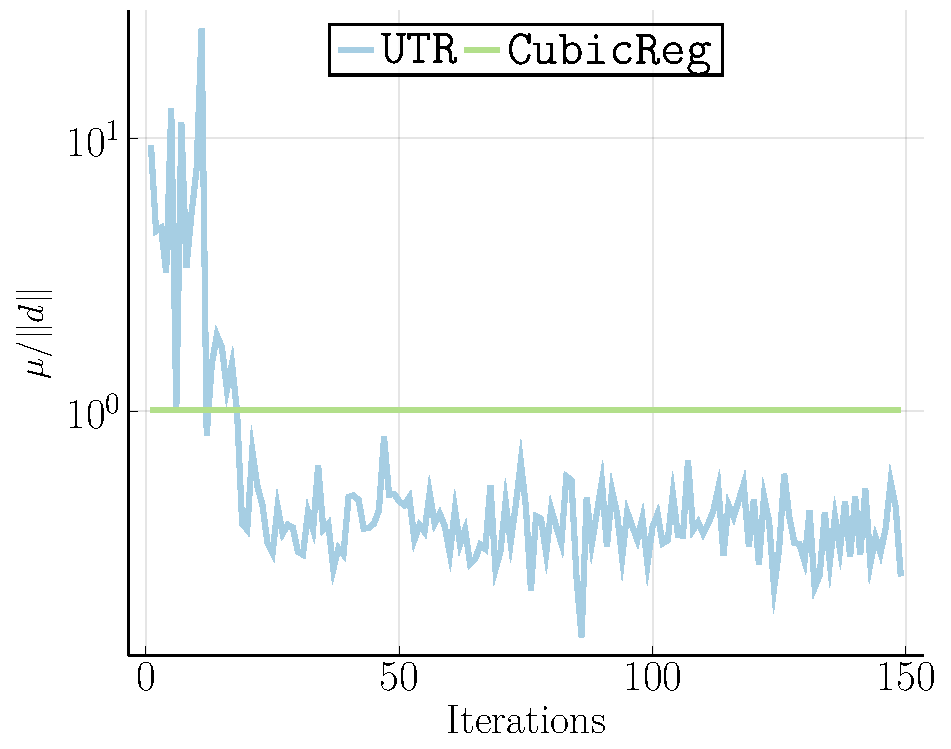
\includegraphics[width=0.9\columnwidth]{figs/ratio.pdf}
    \caption{The ratio of $\mu/\|d\|$ for a typical trust-region method and the cubic Newton method.}
    \label{fig.soft maximum ratio}
\end{figure}

In contrast, for the cubic Newton method, such regularity condition always holds since the optimality condition of the subproblem \eqref{eq.cr update} gives
\begin{equation*}
    \left (\nabla^2 f(x) + \frac{M}{2}\|d\| I \right )d = -\nabla f(x),
\end{equation*}
and therefore $\mu = \frac{M}{2}\|d\|$ and the regularity condition holds by Lemma~\ref{lem.inner product g and d}.

Fortunately, although this favorable regularity condition is not inherently guaranteed for trust-region-type methods, there is a way to overcome this challenge. Specifically, with careful choice of $(\sigma,r)$, the progress made in the subproblem formulation~\eqref{eq.newTR} can be interpreted in two distinct ways. As demonstrated in the following two lemmas: when $\lambda>0$, we achieve a sufficient decrease in the function value; when $\lambda = 0$, we establish a bound on the gradient norm for the next iteration.

\begin{lemma}
    \label{lem.function decrease}
    Suppose Assumption~\ref{assm.main assm} holds and $(d,\lambda) = \operatorname{SA}(x,\sigma,r)$. When $\sigma \geq M r$ and $\lambda>0$, we have
    \begin{equation}
        \label{eq.function decrease advanced}
        f(x+d) \leq f(x)-\frac{1}{2}d^T \nabla^2 f(x) d-\lambda r^2 -\frac{5M}{6} r^3.
    \end{equation}
\end{lemma}

\begin{lemma}
    \label{lem.bound next gradient}
    Suppose Assumption~\ref{assm.main assm} holds and $(d,\lambda)= \operatorname{SA}(x,\sigma,r)$ , when $\lambda=0$, we have
    \begin{equation}
        \label{eq.bound next gradient}
        \|\nabla f(x+d)\| \leq \frac{M}{2}r^2+\sigma r.
    \end{equation}
\end{lemma}
Moreover, we leverage the above characteristics of trust-region methods and design a customized algorithmic design for trust-region-type methods, enabling a compensatory process that allows the steps to be effectively integrated into the acceleration framework, thereby achieving acceleration.

We review this technique in a simplified manner here. The main idea behind the estimating sequence technique is to maintain a dynamic sequence $\{\phi_k(x),A_k,v_k,x_k\}$ to approximate the objective function $f(x)$ from both above and below. In each iteration, we only update $x_k$ and $v_k$, while the auxiliary sequences $\phi_k(x)$ and $A_k$ are used for theoretical analysis and do not explicitly appear in the algorithm. Specifically, the following relations must be satisfied:
\begin{align}
    \label{eq.es relation 1}
     & \mathcal{R}_k^1: \ \phi_k^*  \geq A_k f(x_k), \  \phi_k^*= \phi_k(v_k) =\min_{x\in\mathbb{R}^n}\phi_k(x) \\
    \label{eq.es relation 2}
     & \mathcal{R}_k^2: \ \phi_k(x)\leq A_kf(x)+\phi_0(x), \ \forall x\in\mathbb{R}^n.
\end{align}
By setting $x = x^*$ in \eqref{eq.es relation 2}, it follows from \eqref{eq.es relation 1} and \eqref{eq.es relation 2} that
\begin{equation*}
    f(x_k)-f^* \leq \frac{1}{A_k}\phi_0(x^*).
\end{equation*}
Thus, the algorithm’s complexity is determined by how rapidly $A_k$ grows. For the accelerated cubic Newton method, \citet{nesterov2008accelerating} proposed an efficient way to update the aforementioned sequence and demonstrated that $A_k=\Theta(k^3)$, leading to an iteration complexity of $O(\epsilon^{-1/3})$.

In summary, the estimating sequence technique captures a recursive relationship between the function values across iterations. However, only second-order algorithms whose iterates satisfy the regularity condition can inherit this recursive function value reduction relationship. As mentioned earlier, the trust-region-type methods do not inherently guarantee that this regularity condition holds. This phenomenon highlights the need for a compensatory approach specifically designed to accelerate trust-region-type methods.






% Acknowledgements should only appear in the accepted version.
% \section*{Acknowledgements}

% \textbf{Do not} include acknowledgements in the initial version of
% the paper submitted for blind review.

% If a paper is accepted, the final camera-ready version can (and
% usually should) include acknowledgements.  Such acknowledgements
% should be placed at the end of the section, in an unnumbered section
% that does not count towards the paper page limit. Typically, this will 
% include thanks to reviewers who gave useful comments, to colleagues 
% who contributed to the ideas, and to funding agencies and corporate 
% sponsors that provided financial support.
\section{The Accelerated Trust-Region Method}
In this section, we introduce the Accelerated Trust-Region (ATR) method (Algorithm~\ref{alg.accelerated utr}), along with its auxiliary local detection subroutine Algorithm~\ref{alg.rr}, and provide an explanation of the intuition behind their design.

\begin{algorithm}[ht]
    \caption{Accelerated Trust-Region Method (\atr{})}\label{alg.accelerated utr}
    \begin{algorithmic}[1]
        \STATE \textbf{input:} $x_0=v_0\in \mathbb{R}^n$, $s_0=0$
        \FOR{$k=0, 1, \ldots, K_\epsilon$}
        \STATE $y_k = \frac{k}{k+3}x_k+\frac{3}{k+3}v_k$
        \STATE $(\sigma_k,r_k) = (\frac{\sqrt{M}}{3}\|\nabla f(y_k)\|^{1/2},\frac{1}{3\sqrt{M}}\|\nabla f(y_k)\|^{1/2})$
        \STATE $(d_k,\lambda_k) = \operatorname{SA}(y_k,\sigma_k,r_k)$
        % \noindent\rule{8cm}{0.4pt} 
        \IF{$\lambda_k>0$} \label{line.if}
        % \STATE $x_{k+1}=y_k+d_k$ \label{line.nonzero multiplier}
        \STATE \textbf{\# Case 1: Function Value Decrease}
        \STATE $x_{k+1}=y_k+d_k$
        \STATE $s_k = s_{k-1}+\frac{(k+1)(k+2)}{2}\nabla f(y_k)$
        \ELSE \label{line.else}
        \STATE \textbf{\# Case 2: Local Detection}
        \STATE $d_k = \operatorname{LD}(y_k,d_k)$
        \STATE $x_{k+1}=y_k+d_k$
        \STATE $s_k = s_{k-1}+\frac{(k+1)(k+2)}{2}\nabla f(x_{k+1})$
        \ENDIF
        \STATE $v_{k+1} = v_0-\sqrt{\frac{\ell}{3M\|s_k\|}}s_k$
        \ENDFOR
    \end{algorithmic}
\end{algorithm}

\begin{algorithm}[ht]  \caption{Local Detection for ATR}\label{alg.rr}
    \begin{algorithmic}[1]
        \STATE \textbf{Input: } $y_k,d_k^{(-1)} := d_k\in\mathbb{R}^n$
        \FOR{$j= 0,1,\ldots,\infty$}
        \STATE \textbf{\# Phase 1: Linear Contraction}
        \STATE $\xi^{(j)} = \|\nabla f(y_k+d_k^{(j-1)})\|^{1/2}$
        \IF{$\xi^{(j)}\leq \epsilon$}
        \STATE \textbf{early terminate}
        \ENDIF
        \STATE $(\sigma_k^{(j)},r_k^{(j)}) = (\frac{\sqrt{M}}{3}\xi^{(j)},\frac{1}{3\sqrt{M}}\xi^{(j)})$
        \STATE $(d_k^{(j)},\lambda_k^{(j)})=\operatorname{SA}(y_k,\sigma_k^{(j)},r_k^{(j)})$
        \STATE \textbf{\# Phase 2: Regularity Refinement}
        \IF{$0<\lambda_k^{(j)}\leq \frac{\sqrt{M}}{3}\xi^{(j)}$} \label{line.bisection}
        \STATE \textbf{output } $d_k^{(j)}$ \label{line.zero multiplier 1}
        \ELSIF{$\lambda_k^{(j)}> \frac{\sqrt{M}}{3}\xi^{(j)}$}
        \STATE $\mu_- = \frac{\sqrt{M}}{3}\xi^{(j)}, \mu_+ = \lambda_k^{(j)}+\frac{\sqrt{M}}{3}\xi^{(j)}$ \label{line.bracketing}
        \STATE $d_k^{(j)} = \operatorname{BISECTION}(y_k,\mu_-,\mu_+)$ \label{line.zero multiplier 2}
        \STATE \textbf{output } $d_k^{(j)}$
        \ENDIF \label{line.endbisection}
        \ENDFOR
    \end{algorithmic}
\end{algorithm}

\begin{algorithm}[!ht]
    \caption{Bisection for ATR}\label{alg.bisection}
    \begin{algorithmic}[1]
        \STATE{\textbf{input:} $y\in \mathbb{R}^n$, $\mu_- < \mu_+$;}
        \WHILE{True}
        \STATE{$\mu = \frac{\mu_-+\mu_+}{2}$}
        \STATE{$d = -\left (\nabla ^2 f(y)+\mu I\right )^{-1}\nabla f(y)$}
        \IF{$\frac{\mu}{\|d\|}<M$}
        \STATE{$\mu_-=\mu$}
        \ELSIF{$\frac{\mu}{\|d\|}>2M$}
        \STATE{$\mu_+ = \mu$}
        \ELSE
        \STATE{\textbf{output} $d$}
        \ENDIF
        \ENDWHILE
    \end{algorithmic}
\end{algorithm}

We begin by clarifying Algorithm~\ref{alg.accelerated utr}, which governs the recursive relations in \eqref{eq.es relation 1} and \eqref{eq.es relation 2}. Following the guidance provided by Lemma~\ref{lem.function decrease} and Lemma~\ref{lem.bound next gradient}, a natural approach is to classify the iterations into two cases and handle them separately: one case where the multiplier is nonzero, which sufficiently decreases the function value, and another where the multiplier is zero, resulting in a contraction of the gradient norm. In these two scenarios, we adopt distinct strategies for updating the elements $x_k$ and $v_k$ in the estimating sequence to ensure that the recursive relation transitions smoothly to the next iteration. This distinction is the key difference between our algorithm and other acceleration frameworks.

Specifically, in \textbf{Case 1} of Algorithm~\ref{alg.accelerated utr}, the multiplier $\lambda_k>0$, which means our choice of $\sigma_k,r_k$ has brought a sufficient decrease in function value for the recursive relation to pass down to the next iterate:
\begin{corollary}\label{coro.function value decrease}
    Suppose Assumption~\ref{assm.main assm} holds, in Case~1 of Algorithm~\ref{alg.accelerated utr}, we have
    \begin{equation}
        \label{eq.decrease of order 1.5}
        f(x_{k+1}) \leq f(y_k)-\frac{5}{162\sqrt{M}}\|\nabla f(y_k)\|^{3/2}.
    \end{equation}
\end{corollary}
Therefore, we can skip the regularity condition verification and directly update the estimate sequence in this case.

However, \textbf{Case 2} of Algorithm~1 calls for different processing. We design a 'Local Dection'(LD) process to deal with this case. Specifically, we use Algorithm~\ref{alg.rr} to investigate the local property of the current iterate $y_k$, whose goal is twofold.

On one hand, in \textbf{Phase 1} of Algorithm~\ref{alg.rr}, a distinctive feature is that the gradient norm of the next iterate will keep contracting as long as the multiplier $\lambda_k^{(j)}=0$. Therefore, intuitively, we want to use such contraction to speed up the convergence. In particular, in Algorihtm~\ref{alg.rr} we use the notation $\xi^{(j)}$ to keep track of such contraction.
\begin{corollary}
    \label{coro.inner loop bound next gradient}
    Suppose Assumption~\ref{assm.main assm} holds, if in the $j$-th iteration, Algorithm~\ref{alg.rr} does not output $d_k^{(j)}$ or terminate, then
    \begin{equation}
        \label{eq.inner loop bound next gradient}
        \left(\xi^{(j+1)}\right)^2 \leq \frac{1}{6}\left(\xi^{(j)}\right)^2.
    \end{equation}
\end{corollary}
If such a situation keeps appearing, we will end up with an $\epsilon$-approximate solution and the algorithm is early terminated.

On the other hand, if the multiplier no longer equals zero, we turn to \textbf{Phase 2} to find a step $d_k^{(j)}$ with regularity condition holds. At the beginning of this phase, we are provided with a solution $d_k^{(j)}$ and an interval $[\mu_-,\mu_+]$ for which the regularity condition roughly holds.
\begin{equation*}
    \begin{aligned}
         & \|d_k^{(j)}\| = \frac{1}{3\sqrt{M}}\xi^{(j)}, \\
         & \mu_- = \frac
        {\sqrt{M}}{3}\xi^{(j)}, \ \mu_+= \lambda_k^{(j)} + \frac{\sqrt{M}}{3}\xi^{(j)}.
    \end{aligned}
\end{equation*}
Hence the rest for us to do is to use the above 'good predict' to find a pair of $(d_k,\mu_k)$ such that the regularity condition strictly holds. Luckily, a standard bisection search procedure (Algorithm~\ref{alg.bisection}) can serve this purpose.

Our accelerated Algorithm~\ref{alg.accelerated utr} is capable of automatically adjusting the iteration process based on the local properties of the current point, offering tailored methods for different local characteristics.
\section{Convergence Analysis}
In this section, we analyze the complexity of Algorithm~\ref{alg.accelerated utr}. Let $K_\epsilon$ denote the index of the first iterate that satisfies Definition~\ref{def.approximate solution}. We will show that the number of iterations needed is $K_\epsilon = O(\epsilon^{-1/3})$, and the number of trust-region-subproblems solved within these iterations is bounded by $\tilde{O}(\epsilon^{-1/3})$. We note that, in the worst-case scenario, an additional logarithmic number of trust-region subproblems may need to be solved. However, since the Hessian and gradient of these subproblems remain the same, the additional computational cost is minimal.

First, we formally divide the iterates produced by Algorithm~\ref{alg.accelerated utr} into two sets:
\begin{equation}
    \label{eq.outer index catagory}
    \begin{aligned}
         & \mathcal{N} = \left \{ k | k\leq K_\epsilon,\ x_k \text{\ updated in \textbf{Case 1} of Algorithm~\ref{alg.accelerated utr}}\right\}, \\
         & \mathcal{Z} = \left \{k |k\leq K_\epsilon,\ x_k \text{\ updated in \textbf{Case 2} of Algorithm~\ref{alg.accelerated utr}}\right\}.
    \end{aligned}
\end{equation}
We clarify that there are two ways of finding an $\epsilon$-approximate solution in our algorithm as discussed in the previous section. The first way is that in \textbf{Case 2}, i.e., $k\in\mathcal{Z}$, there is a possibility that the gradient norm keeps contracting until a solution $y_k+d_k^{(j)}$ with $\|\nabla f(y_k+d_k^{(j)})\| \leq \epsilon$ is found. We call Algorithm~\ref{alg.accelerated utr} early terminated in this case. The second way is that Algorithm~\ref{alg.rr} always gives a step $d_k^{(j)}$ with regularity condition holds, and the recursive relation passes down to the next iteration and we can use the estimating sequence to find a solution $x_k$ with $f(x_k)-f^*\leq \epsilon$.

The logic of the proof is that if the first way does not work before $K_\epsilon = O(\epsilon^{-1/3})$-th out iteration, the estimate sequence technique can guarantee that we find an approximate solution. Otherwise, Algorithm~\ref{alg.accelerated utr} is early terminated before $K_\epsilon$-th iteration.

We first examine the complexity of Algorithm~\ref{alg.rr} in each iteration $k$ of Algorithm~\ref{alg.accelerated utr}, the following lemma shows that either Algorithm~\ref{alg.rr} enters \textbf{Phase 2} in a logarithmic complexity or Algorithm~\ref{alg.accelerated utr} is early terminated.

\begin{lemma}
    \label{lem.inner loop terminate}
    In the $k$-th outer loop of Algorithm~\ref{alg.accelerated utr}, Algorithm~\ref{alg.rr} will enter \textbf{Phase 2} in
    \begin{equation*}
        j_k \leq O\left (\log \frac{\|\nabla f(y_k)\|}{\epsilon}\right)
    \end{equation*}
    iterations, otherwise we find an approximate solution in \textbf{Phase 1} such that
    \begin{equation*}
        \| \nabla f(y_k+d_k^{(j_k)})\| \leq \epsilon.
    \end{equation*}
    % Since the inner loop will terminate eventually, we can actually have a tighter bound for $j_k$:
    % \begin{equation}
    %     \label{eq.tighter bound jk}
    %     j_k \leq O\left (\log \frac{\|\nabla f(y_k)\|}{\|\nabla f(y_k+d_k^{(j_k-1)})\|}\right)
    % \end{equation}
\end{lemma}

When Algorithm~\ref{alg.rr} enters \textbf{Phase 2}, our goal is to find a step with regularity condition holds, by Lemma~\ref{lem.inner product g and d}, it is sufficient to find a pair of $\mu_k,d_k$ with $\mu_k = \Theta(\|d_k\|)$. In particular, our choice of parameters in Algorithm~\ref{alg.rr} and Algorithm~\ref{alg.bisection} target at finding
\begin{equation}\label{eq.goal of bisection 1}
    M\|d_k\| \leq \mu_k\leq 2M\|d_k\|,
\end{equation}
we define the auxiliary function for iteration $k$,
\begin{equation}\label{eq.auxiliary bisection function}
    g_{y_k}(\mu): = \frac{\mu}{\|\left(\nabla^2 f(y_k)+\mu I\right)^{-1}\nabla f(y_k)\|}.
\end{equation}
Therefore, the goal \eqref{eq.goal of bisection 1} is equivalent to
\begin{equation}
    \label{eq.goal of bisection 2}
    M\leq g_{y_k}(\mu)\leq 2M.
\end{equation}
The following lemma claims that we have found the bracketing points for the bisection procedure at line~\ref{line.bracketing}.

\begin{lemma}\label{lem.valid bracketing}
    \label{eq.valid bracketing}
    In the $k$-th iteration, in \textbf{Phase 2} of Algorithm~\ref{alg.rr},
    \begin{equation*}
        g_{y_k}(\mu_-) < M, \ g_{y_k}(\mu_+) >2M.
    \end{equation*}
\end{lemma}

Also, to guarantee the validity of the bisection search, we establish the following propositions of $g_{y_k}(\mu)$ over the interval $\left[\mu_-,\mu_+\right]$.
\begin{lemma}
    \label{lem.property g}
    For any $k\geq0$, $g_{y_k}(\mu)$ is continuously differentiable and monotonically increasing for $\mu \in \left (0,+\infty\right ]$. Moreover, its derivative is uniformly bounded above.
\end{lemma}
The above lemmas are crucial in analyzing the complexity of the bisection procedure, with the help of them we have
\begin{lemma}
    \label{lem.bound initial interval}
    At the $k$-th iteration of Algorithm~\ref{alg.accelerated utr}, the complexity of the bisection search procedure is at most $O(\log \frac{\|\nabla f(y_k)\|}{\epsilon})$.
\end{lemma}

As observed, both \textbf{Phase 1} and \textbf{Phase 2} have a complexity of $\log\left(\frac{\|\nabla f(y_k)\|}{\epsilon}\right)$, in \textbf{Phase 1} we need to solve trust-region subproblems while in \textbf{Phase 2} we only need to solve linear equations. We remark that it is more expensive to solve trust-region subproblem than linear equations. Therefore, the complexity of \textbf{Phase 2} is dominated by the complexity of \textbf{Phase 1}. Also, all these trust-region subproblems and linear equations share the same Hessian and the gradient. Which means if we use matrix decomposition, the decomposition is a one-time effort.

Now it remains to bound the gradient norm of the sequence $y_k$ for $k\in \mathcal{Z}$. Fortunately, this can be guaranteed by the following lemma:

\begin{lemma}
    \label{lem.upper bound for zero lambda}
    Suppose Assumption~\ref{assm.main assm} and Assumption~\ref{assm.bounded hessian} hold, for $k\in \mathcal{Z}$, we have
    \begin{equation}
        \label{eq.upper bound for zero lambda}
        \|\nabla f(y_k)\|\leq \frac{9\kappa_H^2}{64M}.
    \end{equation}
    As a consequence, in each iteration of Algorithm~\ref{alg.accelerated utr}, the complexity of Algorithm~\ref{alg.rr} is bounded by $O\left(\log\left(\frac{\kappa_H}{M\epsilon}\right)\right)$
\end{lemma}

Next, we will show how we update the implicit auxiliary sequence $A_k$ and $\phi_k(x)$ and show that $x_k,v_k$ updated in both cases of Algorithm~\ref{alg.accelerated utr} satisfies the recursive relation defined before. Our approach is different from the standard one introduced in~\citet{nesterov_lectures_2018}, mainly in that we update the estimate function sequence $\phi_k(x)$ based on the proposition of the iteration and thus more tailored for trust-region-type methods.

We recursively define
\begin{align}
    \label{eq.update a and A}
     & a_k = \frac{(k+1)(k+2)}{2}, \ A_k=\frac{k(k+1)(k+2)}{6} \\
    \label{eq.update phi}
     & \phi_0(x) = \frac{M}{\ell}\|x-x_0\|^3,
\end{align}
For $k\in\mathcal{N}$,
\begin{equation}\label{eq.update phi 1}
    \phi_{k+1}(x) =\phi_k(x)+a_k\left (f(x_k)+\langle \nabla f(x_k),x-x_k\rangle \right),
\end{equation}
For $k\in\mathcal{Z}$,
\begin{equation}\label{eq.update phi 2}
    \phi_{k+1}(x) =\phi_k(x)+a_k\left (f(y_k)+\langle \nabla f(y_k),x-y_k\rangle \right ),
\end{equation}

The sequences defined above and the iterates produced by Algorithm~\ref{alg.accelerated utr} satisfy the following propositions:
\begin{lemma}
    \label{lem.property of phi}
    For the function sequence $\phi_k(x)$, they have the following properties
    \begin{enumerate}
        \item $v_k$ is the unique minimizer of $\phi_k(x)$, i.e.,
              \begin{equation*}
                  \phi_k^* =\min \phi_k(x) = \phi_k(v_k).
              \end{equation*}
        \item Suppose Assumption~\ref{assm.main assm} holds, set $0<\ell\leq \frac{25}{34992}$, if Algorithm~\ref{alg.accelerated utr} does not early terminate, then $\mathcal{R}_k^1$ and $\mathcal{R}_k^2$ defined in \eqref{eq.es relation 1} and \eqref{eq.es relation 2} hold for all $k\geq0$.
    \end{enumerate}
\end{lemma}

As a direct consequence of the above lemma, the complexity of Algorithm~\ref{alg.accelerated utr} follows,

\begin{theorem}
    \label{thm.convergence outer loop}
    Suppose Assumption~\ref{assm.solvable}, Assumption~\ref{assm.main assm}, and Assumption~\ref{assm.bounded hessian} holds, then Algorithm~\ref{alg.accelerated utr} find an approximate solution satisfies Definition~\ref{def.approximate solution} in $K_\epsilon = O(\epsilon^{-1/3})$ iterations. Moreover, the number of the trust-region subproblems solved is bounded by $\tilde O(\epsilon^{-1/3})$.
\end{theorem}
\section{Numerical Experiments}\label{sec.experiments}
In this section, we implement our accelerated Trust-Region method (\atr{}), to compare with the universal trust-region method (\utr{}, \citet{jiang2024nonconvexityuniversaltrustregionmethod}) which targets at convex optimization, the cubic regularization method (\arc{}, \citet{nesterov2006cubic}) and its accelerated version (\arca{}, \citet{nesterov2008accelerating}). We conduct experiments on the Nesterov's worst case function~\cite{nesterovImplementableTensorMethods2021} and the softmax minimization, which are briefly introduced here; further details and the exact experimental setup can be found in Appendix~\ref{sec.experiments.details}. All experiments are conducted on a single machine with a 14-core Apple M4 Pro CPU  and 48GB LPDDR5 RAM.

We begin by testing performance on Nesterov's worst case function:
\[
    f_k(x) = \eta_{p+1}\left(A_k x\right) - \left\langle e_1, x\right\rangle, \quad 2 \leq p \leq k,
\]
where $\eta_{p+1}(x) = \tfrac{1}{p+1}\|x\|_{p+1}^{p+1}$, and $A_k$ is a parametrized bidiagonal matrix (details in \Cref{sec.experiments.nesterov}). This function becomes increasingly challenging as \(k\) increases.

\begin{figure}[h!]
    \small
    \centering
    \subcaptionbox{$k = 50$}{
        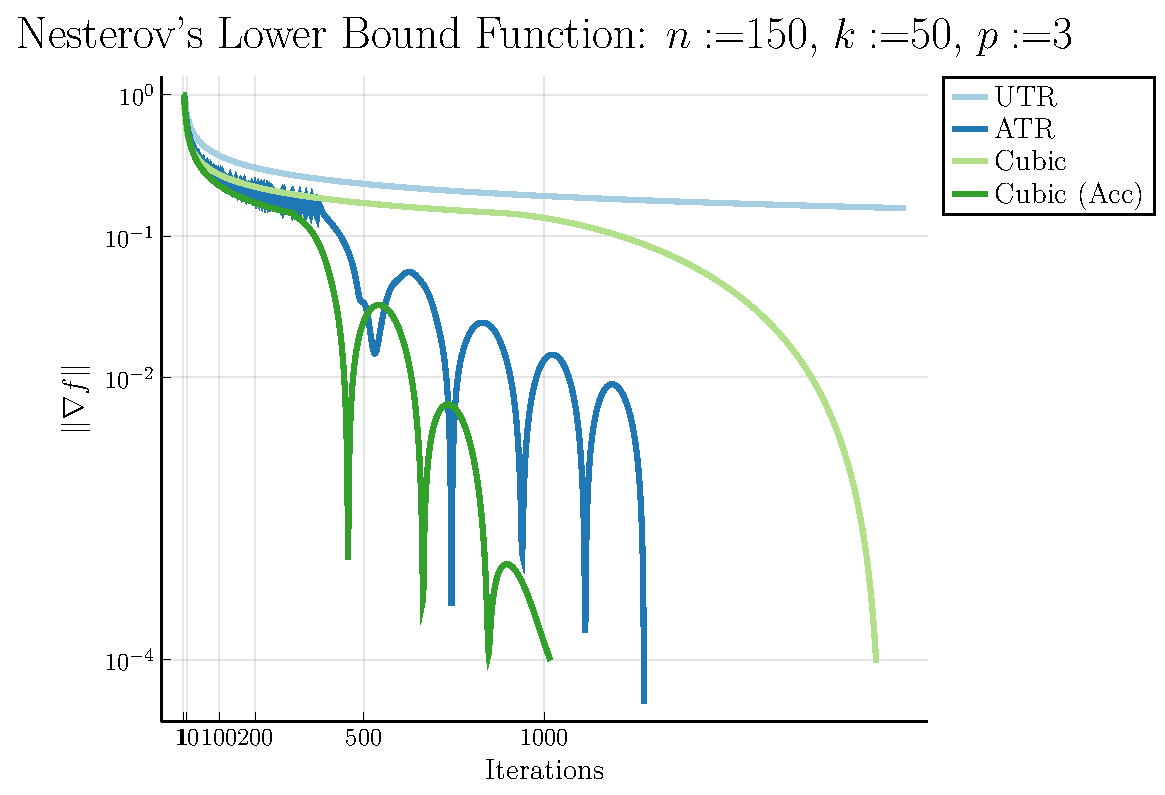
\includegraphics[width=0.47\columnwidth]{figs/e-nesterov-k1.pdf}
    }
    \subcaptionbox{$k = 100$}{
        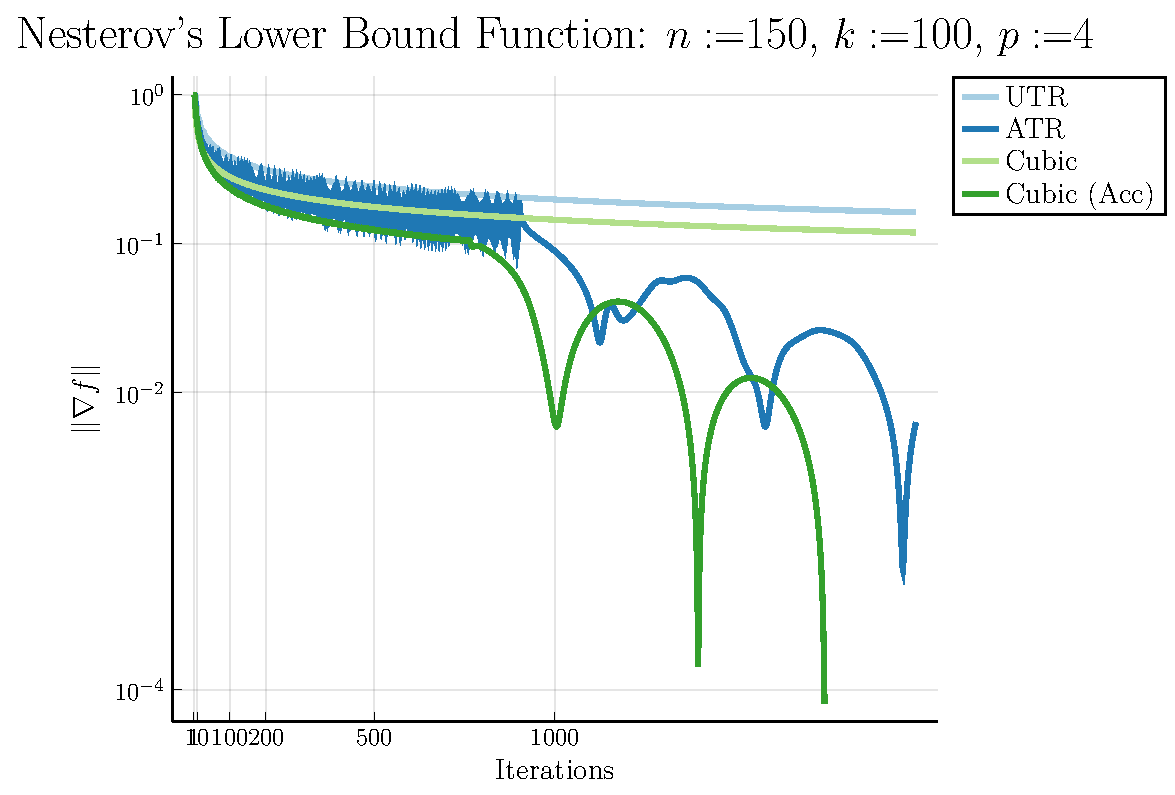
\includegraphics[width=0.47\columnwidth]{figs/e-nesterov-k2.pdf}
    }
    \caption{Nesterov's lower bound problem, $n = 150$, $p = 2$.}\label{fig.nesterov}
    \normalsize
\end{figure}

For this experiment, we fix the problem size and differentiability order, considering \(k = 50, 100\). As shown in \Cref{fig.nesterov}, accelerated methods outperform their original variants, with \atr{} slightly outperforming \arca{} in both cases.

Next, we consider softmax minimization, which approximates piecewise linear functions:
\[
    f(x) := \mu \ln \left(\sum_{i=1}^m \exp \left(\tfrac{a_i^Tx - b_i}{\mu}\right)\right) \approx \max_{1 \leq i \leq m} \left\{a_i^T x - b_i\right\}.
\]
When \(\mu\) is small, this problem is notoriously challenging for unaccelerated methods due to the large smoothness constant, where \(M \leq \tfrac{12}{\mu^2}\) \cite{doikov_super-universal_2024}.

\begin{figure}[h!]
    \small
    \centering
    \subcaptionbox{Iterations}{
        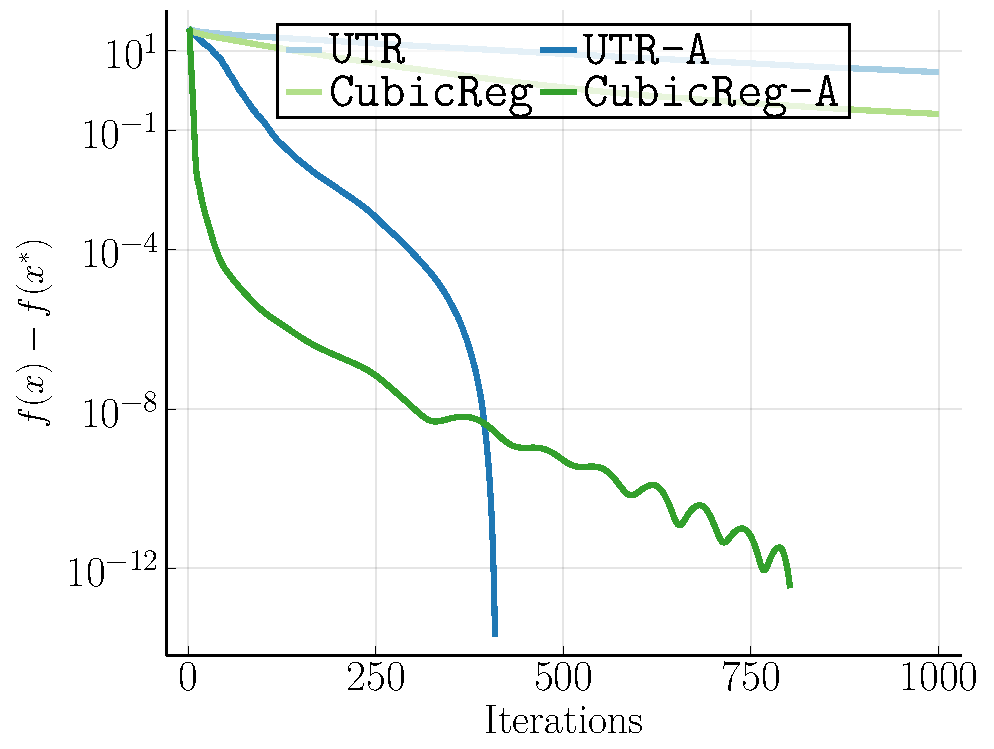
\includegraphics[width=0.47\columnwidth]{figs/fx-softmax-k.pdf}
    }
    \subcaptionbox{Runtime (seconds)}{
        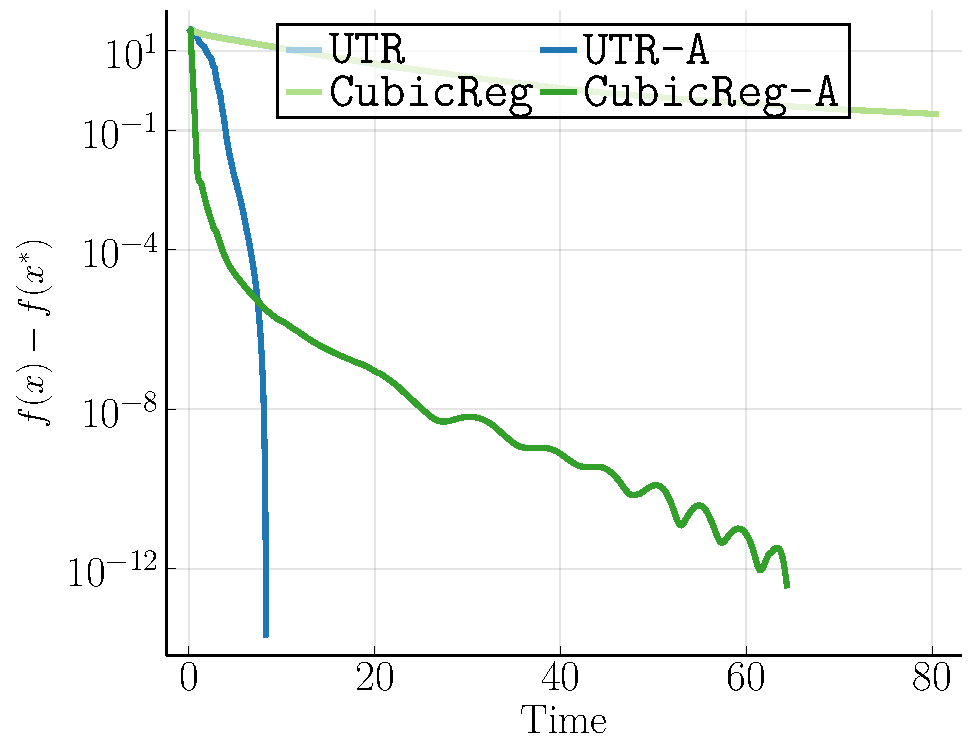
\includegraphics[width=0.47\columnwidth]{figs/fx-softmax-t.pdf}
    }
    \caption{Softmax minimization, $n = 500$, $m = 1000$, $\mu = 0.1$.}\label{fig.softmax}
    \normalsize
\end{figure}

\Cref{fig.softmax} illustrates the results. In addition to comparing iterations (panel (a)), we also present runtime in seconds (panel (b)). Notably, the \emph{per-iteration time} of \atr{} (0.02 seconds) is only one-fourth of \arca{} (0.08 seconds), primarily because solving the trust-region subproblem is computationally simpler than solving the cubic-regularized subproblem.

\section{Conclusion}
In this work, we addressed the challenge of accelerating trust-region-type methods, bridging the gap between their practical success and theoretical development. By proposing a novel framework that effectively utilizes the progress of both function value reduction and gradient norm contraction, we extended the scope of existing acceleration techniques to accommodate the constrained nature of trust-region subproblems. Numerical experiments further support our theoretical findings.
\section*{Impact Statement}
This paper does not have any potential societal or ethical consequences.


% In the unusual situation where you want a paper to appear in the
% references without citing it in the main text, use \nocite
\nocite{langley00}

\bibliography{example_paper}
\bibliographystyle{icml2025}


%%%%%%%%%%%%%%%%%%%%%%%%%%%%%%%%%%%%%%%%%%%%%%%%%%%%%%%%%%%%%%%%%%%%%%%%%%%%%%%
%%%%%%%%%%%%%%%%%%%%%%%%%%%%%%%%%%%%%%%%%%%%%%%%%%%%%%%%%%%%%%%%%%%%%%%%%%%%%%%
% APPENDIX
%%%%%%%%%%%%%%%%%%%%%%%%%%%%%%%%%%%%%%%%%%%%%%%%%%%%%%%%%%%%%%%%%%%%%%%%%%%%%%%
%%%%%%%%%%%%%%%%%%%%%%%%%%%%%%%%%%%%%%%%%%%%%%%%%%%%%%%%%%%%%%%%%%%%%%%%%%%%%%%
\newpage
\appendix
\onecolumn
\section{Details of Experiments}\label{sec.experiments.details}

We implement \utr{}, \atr{}, \arc{}, and \arca{} in Julia Programming Language. In all algorithms, we have to solve the following canonical subproblem:
\begin{equation}
    \begin{aligned}
        \min_d ~              & \frac{1}{2}d^T\nabla^2 f(x_k)d + \frac{1}{p!}\sigma_k\|d\|^p + \nabla f(x_k)^T d \\
        \operatorname{s.t.} ~ & \|d\| \le r_k.
    \end{aligned}
\end{equation}
where if $p=2$, it is the subproblem in \utr{} and \atr{}; else if $p=3$ and there is no trust-region constraint, it is the subproblem in \arc{} and \arca{}. We implement a unifying procedure to solve the \emph{secant equation}:
\begin{equation}
    d = \left(\nabla^2 f(x_k) + \mu_k I\right)^{-1}\nabla f(x_k)
\end{equation}
where $\mu_k$ is adjusted and each linear system is solved via Cholesky factorization. Our implementation is more competitive to state-of-the-art solvers in terms of iteration numbers and CPU time. For example, we compare iteration numbers and CPU time in \Cref{fig.softmax} to those in \cite{doikov_super-universal_2024}.

Further details of the test problems are provided in the following.
\paragraph{Nesterov's lower bound problem}\label{sec.experiments.nesterov}
Nesterov's lower bound problem \cite{nesterovImplementableTensorMethods2021} is defined as the following:
\[
    f_k(x) = \eta_{p+1}\left(A_k x\right) - \left\langle e_1, x\right\rangle, \quad 2 \leq p \leq k,
\]
where $\eta_{p+1}(x) = \tfrac{1}{p+1}\|x\|_{p+1}^{p+1}$, and $A_k$ is a parametrized bidiagonal matrix, and $e_1$ is the first standard basis vector.
\small
$$A_k=\left[\begin{array}{cc}U_k & 0 \\ 0 & I_{n-k}\end{array}\right], \quad U_k=\left[\begin{array}{rrccr}1 & -1 & 0 & \ldots & 0 \\ 0 & 1 & -1 & \ldots & 0 \\ & & \ldots & \ldots & \\ 0 & 0 & \ldots & 1 & -1 \\ 0 & 0 & \ldots & 0 & 1\end{array}\right]$$
\normalsize
For a $p$-th order method starting at $x_0 = 0$, the lower bound on the rate of convergence is given by
$O\left(k^{-(1.5p+0.5)}\right)$ (Theorem 4, \cite{nesterovImplementableTensorMethods2021}).
\paragraph{Softmax minimization}
The softmax minimization problem is a smooth approximation of the nonsmooth piecewise linear functions:
\[
    f(x) := \mu \ln \left(\sum_{i=1}^m \exp \left(\tfrac{a_i^Tx - b_i}{\mu}\right)\right) \approx \max_{1 \leq i \leq m} \left\{a_i^T x - b_i\right\} =: \ell(x).
\]
where $i$ is the index of data points, $a_i \in \mathbb{R}^n$ and $b_i \in \mathbb{R}$.
It is a valid approximation because that (see, for example, \cite{beckSmoothingFirstOrder2012})
\begin{align*}
    0 \le  f(x) - \ell(x) \le \mu \log(m), \forall x \in \mathbb{R}^n.
\end{align*}
and the approximation error is bounded by $\mu \log(m)$.
\begin{align*}
    f(x) - \inf f(x) \le \epsilon ~\Rightarrow ~ \ell(x) - \ell(x^*) \le \epsilon + \mu \log(m).
\end{align*}
Choosing a small $\mu$ is hard numerically.
It is known that $f(x)$ has a first-order Lipschitz constant $\tfrac{\|A\|_\infty}{\mu}$. In the experiments, we set $m = 1000, n = 500$, all entries of $a_i, i=1,...,m$ are sampled from the uniform distribution on $[-1,1]$. Then the we see for second-order methods, $M \le \tfrac{12}{\mu^2}$.
\section{Missing Proofs}\label{sec.proofs}
In this sections, we provide proofs to the technical lemmas and theorems in the main text. We will provide more formal format of them with order notation replaced with the specific constant.

First, we introduce an important lemma which will be used throughout this section, which is a direct consequence of Assumption~\ref{assm.main assm}:
\begin{lemma}[Lemma 4.1.1, \citet{nesterov_lectures_2018}]\label{lem.lipschitz}
    If \(f:\mathbb{R}^n \mapsto \mathbb{R}\) satisfies \autoref{assm.main assm}, then for all \(x,y\in \mathbb{R}^n\), we have
    \begin{subequations}
        \begin{align}
            \label{eq.first-order exp}
             & \left\|\nabla f(y)-\nabla f(x)-\nabla^{2} f(x)(y-x)\right\|                       \leq \frac{M}{2}\|y-x\|^{2} \\
            \label{eq.second-order exp}
             & \left|f(y)-f(x)-\nabla f(x)^T(y-x)-\frac{1}{2}(y-x)^T\nabla^{2} f(x)(y-x)\right|  \leq \frac{M}{6}\|y-x\|^{3}
        \end{align}
    \end{subequations}
\end{lemma}
\paragraph{Proof to Lemma~\ref{lem.inner product g and d}}
\begin{lemma}
    \label{lem.inner product g and d appendix}
    Suppose Assumption~\ref{assm.main assm} holds, and \eqref{eq.second-order update} holds for some $\mu$ with $\mu\geq M \|d\|$, then we have
    \begin{equation}
        \label{eq.inner product g d appendix}
        \langle \nabla f(x+d),-d \rangle \geq \frac{\|\nabla f(x+d)\|^2}{2\mu}+\frac{3}{8}\mu \|d\|^2.
    \end{equation}
    Further, if $\mu \leq 2M\|d\|$, we have
    \begin{equation}
        \label{eq.inner product g d advanced appendix}
        \langle \nabla f(x+d),-d \rangle \geq \frac{\sqrt{6}}{6} \frac{\|\nabla f(x+d)\|^{3/2}}{\sqrt{M}}.
    \end{equation}
\end{lemma}
\begin{proof}
    Set $y=x+d$ in \eqref{eq.first-order exp}, we have
    \begin{equation*}
        \|\nabla f(x+d)-\nabla f(x)-\nabla ^2 f(x) d\| \leq \frac{M}{2}\|d\|^2.
    \end{equation*}
    Plug \eqref{eq.second-order update} into the above, we have
    \begin{equation*}
        \|\nabla f(x+d)+\mu d\| \leq \frac{M}{2}\|d\|^2.
    \end{equation*}
    Squaring both sides and rearranging items, we have
    \begin{equation*}
        \begin{aligned}
            2\mu \langle \nabla f(x+d),-d \rangle & \geq \|\nabla f(x+d)\|^2 +\mu^2 \|d\|^2 -\frac{M}{4}\|d\|^4 \\
                                                  & \geq \|\nabla f(x+d)\|^2 +\frac{3}{4}\mu^2 \|d\|^2.
        \end{aligned}
    \end{equation*}
    The second line is due to $\mu\geq M\|d\|$, dividing both sides by $2\mu$ gives \eqref{eq.inner product g d appendix}. Further, when $\mu \leq 2M\|d\|$, the above gives
    \begin{equation*}
        4M\|d\| \langle \nabla f(x+d),-d \rangle \geq \|f(x+d)\|^2 +\frac{3}{4} M^2 \|d\|^4,
    \end{equation*}
    which yields
    \begin{equation*}
        \langle \nabla f(x+d),-d \rangle \geq \frac{\|f(x+d)\|^2}{4M\|d\|}+\frac{3}{16}M\|d\|^3.
    \end{equation*}
    Consider an auxiliary function $h(t) = \frac{\|f(x+d)\|^2}{4Mt}+\frac{3}{16}Mt^3$ where $t\geq 0$, taking derivatives gives $h(t)$ achieves its minimum at $t^*= \frac{\sqrt{2}\|\nabla f(x+d)\|^{1/2}}{\sqrt{3M}}$, plugging $t^*$ back gives \eqref{eq.inner product g d advanced appendix}.
\end{proof}
\paragraph{Proof to Lemma~\ref{lem.function decrease}}
\begin{lemma}
    \label{lem.function decrease appendix}
    Suppose \autoref{assm.main assm} holds and $(d,\lambda) = \operatorname{SA}(x,\sigma,r)$, then we have
    \begin{equation}
        \label{eq.function decrease appendix}
        f(x+d) \leq f(x) -\frac{1}{2}d^T \nabla^2 f(x) d -(\lambda+\sigma)\|d\|^2 +\frac{M}{6}\|d\|^3.
    \end{equation}
    Especially, when $\sigma \geq M r$ and $\lambda>0$, we have
    \begin{equation}
        \label{eq.function decrease advanced appendix}
        f(x+d) \leq f(x)-\frac{1}{2}d^T \nabla^2 f(x) d-\lambda r^2 -\frac{5M}{6} r^3.
    \end{equation}
\end{lemma}
\begin{proof}
    Set $y=x+d$ in \eqref{eq.second-order exp}, we have
    \begin{equation*}
        f(x+d) \leq f(x) +\nabla f(x)^T d +\frac{1}{2}d^T \nabla ^2 f(x) d +\frac{M}{6}\|d\|^3.
    \end{equation*}
    Plug \eqref{eq.optcond firstorder} into the above we have \eqref{eq.function decrease appendix}. Note that when $\lambda>0$, from \eqref{eq.optcond coml slack} we have $\|d\| = r$, from \eqref{eq.function decrease appendix}, we have
    \begin{equation*}
        \begin{aligned}
            f(x+d) & \leq f(x)-\frac{1}{2}d^T \nabla^2 f(x)d-\lambda r^2-\sigma r^2+\frac{M}{6}r^3 \\
                   & \leq f(x)-\frac{1}{2}d^T \nabla^2 f(x) d-\lambda r^2 -\frac{5M}{6} r^3.
        \end{aligned}
    \end{equation*}
    In the second line, we used $\sigma \geq M r.$
\end{proof}
\paragraph{Proof to Lemma~\ref{lem.bound next gradient}}
\begin{lemma}
    \label{lem.bound next gradient appendix}
    Suppose \autoref{assm.main assm} holds and $(d,\lambda)= \operatorname{SA}(x,\sigma,r)$ , then we have
    \begin{equation}
        \label{eq.bound next gradient appendix}
        \|\nabla f(x+d)\| \leq \frac{M}{2}r_k^2+(\sigma_k+\lambda_k)r_k.
    \end{equation}
\end{lemma}
\begin{proof}
    From \eqref{eq.second-order exp}, we have
    \begin{equation*}
        \|\nabla f(x+d)- \nabla f(x) -\nabla ^2 f(x) d\| \leq \frac{M}{2}\|d\|^2.
    \end{equation*}
    By \eqref{eq.optcond firstorder} and the above, we have
    \begin{equation*}
        \|\nabla f(x+d)+(\sigma+\lambda) d\| \leq \frac{M}{2}\|d\|^2.
    \end{equation*}
    Note $\|d\|\leq r$, apply the triangle inequality and rearrange items we can derive \eqref{eq.bound next gradient appendix}.
\end{proof}
\paragraph{Proof to Corollary~\ref{coro.function value decrease}}
\begin{corollary}\label{coro.function value decrease appendix}
    Suppose Assumption~\ref{assm.main assm} holds, in Case~1 of Algorithm~\ref{alg.accelerated utr}, we have
    \begin{equation}
        \label{eq.decrease of order 1.5 appendix}
        f(x_{k+1}) \leq f(y_k)-\frac{5}{162\sqrt{M}}\|\nabla f(y_k)\|^{3/2}.
    \end{equation}
\end{corollary}
\begin{proof}
    Note $\nabla^2 f(x)\succeq 0$. This is a direct consequence of plugging $x=y_k$, $x+d =x_{k+1}= y_k+d_k$, and $(\sigma,r) = (\frac{\sqrt{M}}{3}\|\nabla f(y_k)\|^{1/2},\frac{1}{3\sqrt{M}}\|\nabla f(y_k)\|^{1/2})$ into Lemma~\ref{lem.function decrease appendix}.
\end{proof}
\paragraph{Proof to Corollary~\ref{coro.inner loop bound next gradient}}
\begin{corollary}
    \label{coro.inner loop bound next gradient appendix}
    Suppose Assumption~\ref{assm.main assm} holds, if in the $j$-th iteration, Algorithm~\ref{alg.rr} does not output $d_k^{(j)}$ or terminate, then
    \begin{equation}
        \label{eq.inner loop bound next gradient appendix}
        \left(\xi^{(j+1)}\right)^2 \leq \frac{1}{6}\left(\xi^{(j)}\right)^2.
    \end{equation}
\end{corollary}
\begin{proof}
    This is a direct consequence of $\lambda_k^{(j)}=0$ and plugging $x+d = y_k+d_k^{(j)}$, $(\sigma,r) = \left(\frac{\sqrt{M}}{3}\xi^{(j)},\frac{1}{3\sqrt{M}}\xi^{(j)}\right)$ into \eqref{eq.bound next gradient appendix}.
\end{proof}
\paragraph{Proof to Lemma~\ref{lem.inner loop terminate}}
\begin{lemma}
    \label{lem.inner loop terminate appendix}
    In the $k$-th outer loop of Algorithm~\ref{alg.accelerated utr}, Algorithm~\ref{alg.rr} will enter \textbf{Phase 2} in
    \begin{equation*}
        j_k \leq O\left (\log \frac{\|\nabla f(y_k)\|}{\epsilon}\right)
    \end{equation*}
    iterations, otherwise we find a point such that
    \begin{equation*}
        \| \nabla f(y_k+d_k^{(j_k)})\| \leq \epsilon.
    \end{equation*}
\end{lemma}
\begin{proof}
    Note that if in \textbf{Phase 1}, the multiplier $\lambda_k^{(j)}$ keeps being equal to $0$, the gradient norm will keep contracting as \eqref{eq.inner loop bound next gradient appendix} is equivalent to
    \begin{equation*}
        \|\nabla f(y_k+d_k^{(j)})\|\leq \frac{1}{6}\|\nabla f(y_k+d_k^{(j-1)})\|.
    \end{equation*}
    Then in $O\left (\log \frac{\|\nabla f(y_k)\|}{\epsilon}\right)$ iterations, we either have terminated the algorithm with an approximate solution found or Algorithm~\ref{alg.rr} enters \textbf{Phase 2}.
\end{proof}
\paragraph{Proof to the Complexity of the Bisection Procedure}
Since both Lemma~\ref{lem.valid bracketing}-\ref{lem.bound initial interval} are intermediate, we proof them altogether to derive the complexity of the bisection procedure.

Suppose in the $k$-th iteration of Algorithm~\ref{alg.accelerated utr}, the Local detection subroutine Algorithm~\ref{alg.rr} enters the bisection procedure at the $j_k$-th inner iteration, then by the mechanism of Algorithm~\ref{alg.rr}, the following can be established:
\begin{gather}
    \label{eq.magnitude lambda}
    \lambda_k^{(j_k)} > \frac{\sqrt{M}}{3}\|\nabla f(y_k+d_k^{(j_k-1)})\|^{1/2}\\
    \label{eq.set mu plus}
    \mu_+ = \lambda_k^{(j_k)}+\frac{\sqrt{M}}{3}\|\nabla f(y_k+d_k^{(j_k-1)})\|^{1/2}> \frac{2\sqrt{M}}{3}\|\nabla f(y_k+d_k^{(j_k-1)})\|^{1/2}\\
    \label{eq.newton equation}
    \left (\nabla ^2 f(y_k)+\mu_+ I\right) d_k^{(j_k)}=-\nabla f(y_k)\\
    \label{eq.step size}
    \|d_k^{(j_k)}\| = \frac{1}{3\sqrt{M}}\|\nabla f(y_k+d_k^{(j_k-1)})\|^{1/2}.
\end{gather}

We first review the mission of the bisection procedure: for the auxiliary function $g_{y_k}(\mu) = \frac{\mu}{\|\left (\nabla^2 f(y_k)+\mu I\right)^{-1}\nabla f(y_k)\|}$, given current point $y_k$, our goal is to find the regularize $\mu$ such that
\begin{equation*}
    M \leq g_{y_k}(\mu) \leq 2M.
\end{equation*}
We first analyze some basic properties of $g_{y_k}(\mu)$,
\begin{lemma}
    \label{lem.property g appendix}
    For any $y_k\in \mathbb{R}^n$, $g_{y_k}(\mu)$ is continuously differentiable and monotonically increasing for $\mu \in \left (0,+\infty\right ]$ and
    \begin{equation}
        \label{eq.derivative}
        g_{y_k}'(\mu) = \frac{1}{\|\left (\nabla ^2 f(y_k)+\mu I \right)^{-1}\nabla f(y_k)\|}+\frac{\mu}{\|\left (\nabla ^2 f(y_k)+\mu I \right)^{-1}\nabla f(y_k)\|^3}\sum_{i=1}^n\frac{\beta_i^2}{\left (\lambda_i+\mu\right )^3},
    \end{equation}
    and it is bounded both below and above
    \begin{equation}
        \label{eq.derivative bound}
        0< g_{y_k}'(\mu) \leq \frac{2}{\|\left (\nabla ^2 f(y_k)+\mu I \right)^{-1}\nabla f(y_k)\|}.
    \end{equation}
    Where $\lambda_i$ is the $i$-th eigenvalue of $\nabla ^2 f(y_k)$, $\beta_i = \nabla f(y_k)^T v_i$, $v_i$ denotes the eigenvector corresponding to $\lambda_i$.
\end{lemma}
\begin{proof}
    Since $\nabla^2 f(y_k)+\mu I \succ 0$ for $\mu>0$, we can apply eigen decomposition to it, then
    \begin{equation*}
        \|\left (\nabla ^2 f(y_k)+\mu I \right)^{-1}\nabla f(y_k)\|=\sqrt{\sum_{i=1}^n \frac{\beta_i^2}{\left (\lambda_i+\mu\right )^2}}, \ g_{y_k}(\mu) = \frac{\mu}{\sqrt{\sum_{i=1}^n \frac{\beta_i^2}{\left (\lambda_i+\mu\right )^2}}}.
    \end{equation*}
    Obviously $g_{y_k}(\mu)$ is increasing in $\mu \in \left (0,+\infty\right ]$. Also, through some basic calculations, we have
    \begin{equation*}
        \begin{aligned}
            g_{y_k}'(\mu) & = \frac{1}{\sqrt{\sum_{i=1}^n \frac{\beta_i^2}{\left (\lambda_i+\mu\right )^2}}}+\mu \frac{1}{\left ( (\sum_{i=1}^n \frac{\beta_i^2}{\left (\lambda_i+\mu\right )^2}\right )^{3/2}}\sum_{i=1}^n\frac{\beta_i^2}{\left (\lambda_i+\mu\right )^3} \\
                          & = \frac{1}{\|\left (\nabla ^2 f(y_k)+\mu I \right)^{-1}\nabla f(y_k)\|}+\frac{\mu}{\|\left (\nabla ^2 f(y_k)+\mu I \right)^{-1}\nabla f(y_k)\|^3}\sum_{i=1}^n\frac{\beta_i^2}{\left (\lambda_i+\mu\right )^3}                                   \\
                          & \leq \frac{1}{\|\left (\nabla ^2 f(y_k)+\mu I \right)^{-1}\nabla f(y_k)\|}+\frac{\mu}{\|\left (\nabla ^2 f(y_k)+\mu I \right)^{-1}\nabla f(y_k)\|^3}\sum_{i=1}^n\frac{\beta_i^2}{\mu\left (\lambda_i+\mu\right )^2}                             \\
                          & =  \frac{2}{\|\left (\nabla ^2 f(y_k)+\mu I \right)^{-1}\nabla f(y_k)\|}.
        \end{aligned}
    \end{equation*}
    The inequality is because of $\lambda_i \geq 0$ for $i=1,\ldots,n$.
\end{proof}
We now show that the choices $\mu_+,\mu_-$ in Algorithm~\ref{alg.rr} are valid for the bisection procedure,
\begin{lemma}\label{lem.valid bracketing appendix}
    \label{eq.valid bracketing appendix}
    In the $k$-th iteration, in \textbf{Phase 2} of Algorithm~\ref{alg.rr},
    \begin{equation*}
        g_{y_k}(\mu_-) < M, \ g_{y_k}(\mu_+) >2M.
    \end{equation*}
\end{lemma}
\begin{proof}
    From the mechanism of Algorithm~\ref{alg.rr}, we have
    \begin{equation*}
        \| \left (\nabla ^2 f(y_k)+\mu^+ I\right )^{-1} \nabla f(y_k)\| = \frac{1}{3\sqrt{M}}\|\nabla f(y_k+d_k^{(j_k-1)})\|^{1/2}, \ \mu_+ >\frac{2\sqrt{M}}{3}\|\nabla f(y_k+d_k^{(j_k-1)})\|^{1/2}=2M\|d_k^{(j_k)}\|,
    \end{equation*}
    thus $g_{y_k}(\mu_+) >2M$. Since $\mu_- <\mu^+$, then
    \begin{equation*}
        \| \left (\nabla ^2 f(y_k)+\mu^- I\right )^{-1} \nabla f(y_k)\|>\| \left (\nabla ^2 f(y_k)+\mu^+ I\right )^{-1} \nabla f(y_k)\| = \frac{1}{3\sqrt{M}}\|\nabla f(y_k+d_k^{(j_k-1)})\|^{1/2},
    \end{equation*}
    therefore $g_{y_k}(\mu_-)< M$.
\end{proof}
From the continuity and monotonicity of $g_{y_k}(\mu)$, we know there exist $\mu_-<\mu_l<\mu_u<\mu_+$ such that
\begin{equation}\label{eq.target interval bracketing points}
    g_{y_k}(\mu_l)=M, \ g_{y_k}(\mu_u)=2M.
\end{equation}
To clarify, now we are given the initial interval $[\mu_-,\mu_+]$ and are using bisection to find some $\mu\in[\mu_l,\mu_u]$, once we establish a lower bound for the length of the target interval then we can bound the complexity for the bisection procedure.
\begin{lemma}
    \label{lem.bound target interval}
    For $\mu_l,\mu_u$ in \eqref{eq.target interval bracketing points}, we have
    \begin{equation}
        \label{eq.bound target interval}
        \mu_u-\mu_l \geq \frac{\sqrt{M}\|\nabla f(y_k+d_k^{(j_k-1)})\|^{1/2}}{6}.
    \end{equation}
\end{lemma}
\begin{proof}
    By the mean value theorem, there exists $\xi\in \left [\mu_l,\mu_u\right]$, such that
    \begin{equation*}
        M=g_{y_k}(\mu_u)-g_{y_k}(\mu_l) = g_{y_k}'(\xi)(\mu_u-\mu_l),
    \end{equation*}
    combine the above with \eqref{eq.derivative bound} and \eqref{eq.target interval bracketing points} we have
    \begin{equation*}
        \begin{aligned}
            \mu_+-\mu_- & =  \frac{1}{g_{y_k}'(\xi)}\left(g_{y_k}(\mu_u)-g_{y_k}(\mu_l)\right)           \\
                        & \geq \frac{M\|\left (\nabla ^2 f(y_k)+\xi I \right )^{-1}\nabla f(y_k)\|}{2}   \\
                        & \geq \frac{M\|\left (\nabla ^2 f(y_k)+\mu_+ I \right )^{-1}\nabla f(y_k)\|}{2} \\
                        & = \frac{\sqrt{M}\|\nabla f(y_k+d_k^{(j_k-1)})\|^{1/2}}{6}.
        \end{aligned}
    \end{equation*}
    The third line is because of $\mu_+ >\xi$, the last line is from \eqref{eq.newton equation} and \eqref{eq.step size}.
\end{proof}
Now we established a lower bound for the target interval, it remains to bound the length of the initial interval $\mu_+ -\mu_- = \lambda_k^{(j_k)}$.
\begin{lemma}
    \label{lem.bound initial interval appendix}
    At the $k$-th iteration of Algorithm~\ref{alg.accelerated utr}, if the Algorithm~\ref{alg.rr} enters \textbf{Phase 2}, we have
    \begin{equation*}
        \lambda_k^{(j_k)}\leq \frac{3\sqrt{M}\|\nabla f(y_k)\|}{\|\nabla f(y_k+d_k^{(j_k-1)})\|^{1/2}}\leq O\left(\log\frac{\|\nabla f(y_k)\|}{\epsilon}\right).
    \end{equation*}
    As a consequence, the complexity of the bisection search procedure is
    \begin{equation}
        \label{eq.complexity bisection}
        O \left (\log \left( \frac{\mu_+-\mu_-}{\mu_u-\mu_l}\right)\right)= O\left (\log \left(\frac{\|\nabla f(y_k)\|}{\|\nabla f(y_k+d_k^{(j_k-1)})\|}\right)\right)
    \end{equation}
\end{lemma}
\begin{proof}
    Note that by the mechanism of Algorithm~\ref{alg.rr}, when bisection begins, we have
    \begin{equation*}
        \|\left (\nabla^2 f(y_k)+\mu_+ I \right)d_k^{(j_k)}\| =\|\nabla f(y_k)\|, \ \|d_k^{(j_k)}\| =\frac{1}{3\sqrt{M}}\|\nabla f(y_k+d_k^{(j_k-1)})\|^{1/2}.
    \end{equation*}
    Note that $\nabla ^2 f(y_k)\succeq 0$, and $\mu_+ \geq \lambda_k^{(j_k)}$, we have
    \begin{equation*}
        \lambda_k^{(j_k)}\|d_k^{(j_k)}\| \leq \|\nabla f(y_k)\|,
    \end{equation*}
    thus
    \begin{equation*}
        \lambda_k^{(j_k)} \leq \frac{\|\nabla f(y_k)\|}{\|d_k^{(j_k)}\|} = \frac{3\sqrt{M}\|\nabla f(y_k)\|}{\|\nabla f(y_k+d_k^{(j_k-1)})\|^{1/2}}.
    \end{equation*}
    Combine the above with \eqref{eq.bound target interval} we have
    \begin{equation*}
        \frac{\mu_+-\mu_-}{\mu_u-\mu_l} \leq \frac{18\|\nabla f(y_k)\|}{\|\nabla f(y_k+d_k^{(j_k-1)})\|}.
    \end{equation*}
    Note that $\|\nabla f(y_k+d_k^{(j_k-1)})\|\geq \epsilon$. Hence the proof is finished.
\end{proof}
\paragraph{Proof to Lemma~\ref{lem.upper bound for zero lambda}}
\begin{lemma}
    \label{lem.upper bound for zero lambda appendix}
    Suppose Assumption~\ref{assm.main assm} and Assumption~\ref{assm.bounded hessian} hold, for $k\in \mathcal{Z}$, we have
    \begin{equation}
        \label{eq.upper bound for zero lambda appendix}
        \|\nabla f(y_k)\|\leq \frac{9\kappa_H^2}{64M}.
    \end{equation}
    As a consequence, in each iteration of Algorithm~\ref{alg.accelerated utr}, the complexity of Algorithm~\ref{alg.rr} is bounded by $O\left(\log\left(\frac{\kappa_H}{M\epsilon}\right)\right)$
\end{lemma}
\begin{proof}
    Note that when $k\in \mathcal{Z}$, we have $\lambda_k =0$, hence the following hold
    \begin{equation*}
        \left (\nabla^2 f(y_k)+\frac{\sqrt{M}}{3}\|\nabla f(y_k)\|^{1/2} I\right )d_k^{(0)} = -\nabla f(y_k), \ \|d_k^{(0)}\| \leq \frac{1}{3\sqrt{M}}\|\nabla f(y_k)\|^{1/2}.
    \end{equation*}
    Therefore, by triangle inequality, it holds that
    \begin{equation*}
        \|\nabla f(y_k)\| \leq \|\nabla^2 f(y_k) d_k^{(0)}\| +\frac{\sqrt{M}}{3}\|\nabla f(y_k)\|^{1/2}\|d_k^{(0)}\| \leq \|\nabla^2 f(y_k) d_k^{(0)}\|+\frac{1}{9}\|\nabla f(y_k)\|.
    \end{equation*}
    By \autoref{assm.bounded hessian}, we have
    \begin{equation*}
        \begin{aligned}
            \kappa_H \cdot \frac{1}{3\sqrt{M}}\|\nabla f(y_k)\|^{1/2} & \geq \kappa_H \|d_k^{(0)}\|        \\
                                                                      & \geq \|\nabla^2 f(y_k) d_k^{(0)}\| \\
                                                                      & \geq \frac{8}{9}\|\nabla f(y_k)\|.
        \end{aligned}
    \end{equation*}
    Rearrange items we will have \eqref{eq.upper bound for zero lambda appendix}.
\end{proof}
\paragraph{Proof to the Total Complexity of Algorithm~\ref{alg.accelerated utr}}
Since the iteration complexity results of Theorem~\ref{thm.convergence outer loop} is a direct consequence of Lemma~\ref{lem.property of phi} and the number of total subproblems solved is a direct consequence of the above Lemma~\ref{lem.inner loop terminate} and the complexity of the bisection search, we will direct prove the main theorem which demonstrates the complexity.

Here are some basic properties of the estimating sequence, which is modified from \citet{nesterov_lectures_2018}.
\begin{lemma}
    \label{lem.magnitude a and A}
    For $k\geq 0$, we have
    \begin{equation}
        \label{eq.magnitude a and A}
        \frac{A_{k+1}}{a_k^{3/2}} \geq \frac{\sqrt{2}}{3}.
    \end{equation}
\end{lemma}
\begin{proof}
    $\frac{A_{k+1}}{a_k^{3/2}}= \frac{(k+1)(k+2)(k+3)}{6}\cdot \frac{2^{3/2}}{(k+1)^{3/2}(k+2)^{3/2}} = \frac{\sqrt{2}(k+3)}{3(k+1)^{1/2}(k+2)^{1/2}} \geq \frac{\sqrt{2}}{3}.$
\end{proof}
We call a differentiable function $d(x)$ on $\mathbb{R}^n$ uniformly convex \citet[Section 4.2.2]{nesterov_lectures_2018} of degree $p\geq 2$ with constant $q>0$ if
\begin{equation}
    \label{eq.uniformly convex of p}
    d(y)\geq d(x)+\langle \nabla d(x),y-x\rangle +\frac{q}{p}\|y-x\|^p, \ \forall x,y\in\mathbb{R}^n.
\end{equation}
\begin{lemma}
    \label{lem.property of phi appendix}
    For the function sequence $\phi_k(x)$, they have the following properties
    \begin{enumerate}
        \item $\phi_k(x)$ is uniformly convex of degree $3$ with constant $\frac{3M}{2\ell}$.
        \item $v_k$ is the unique minimizer of $\phi_k(x)$, and
              \begin{equation}
                  \label{eq.phi_k phi_low}
                  \phi_k(x)\geq \phi_k^* + \frac{M}{2\ell}\|x-v_k\|^3.,
              \end{equation}
              where $\phi_k^* =\min \phi_k(x).$
    \end{enumerate}
\end{lemma}
\begin{proof}
    The first claim is from the definition of $\phi_0$ in \eqref{eq.update phi}, for analysis of uniform convex functions, please refer to \citet[Section 4.2.2]{nesterov_lectures_2018}. For the second claim, we have
    \begin{equation}
        \label{eq.phi recursive}
        \phi_k(x) = \phi_0(x)+\sum_{i\in \mathcal{N}_{k}}a_i\left (f(y_i)+\langle \nabla f(y_i),x-y_i\rangle \right)+\sum_{j\in \mathcal{Z}_{k}}a_j\left (f(x_j)+\langle \nabla f(x_j),x-x_j\rangle \right).
    \end{equation}
    From optimality condition
    \begin{equation*}
        \begin{aligned}
            \nabla \phi_k(x) & = \nabla \phi_0(x)+\sum_{i\in \mathcal{N}_k}a_i\nabla f(y_i)+ \sum_{j\in \mathcal{Z}_k}a_j\nabla f(x_j)                \\
                             & = \frac{3M}{\ell}\|x-x_0\|(x-x_0)+\sum_{i\in \mathcal{N}_k}a_i\nabla f(y_i)+ \sum_{j\in \mathcal{Z}_k}a_j\nabla f(x_j) \\
                             & =0.
        \end{aligned}
    \end{equation*}
    Solving the optimality condition and noticing the way we update $s_k$ gives
    \begin{equation*}
        x = v_0 - \sqrt{\frac{\ell}{3M\|s_{k-1}\|}}s_{k-1},
    \end{equation*}
    which is $v_k$. Then \eqref{eq.phi_k phi_low} comes from the factor that $\phi_k(x)$ is uniformly convex of degree 3.
\end{proof}
During the update of the algorithm, we can show that the following properties hold
\begin{lemma}\label{lem.estimate sequence}
    If we set $0<\ell \leq\frac{25}{12\cdot 54^2}$, then we can guarantee the following for all $k\geq 0$:
    \begin{equation}
        \label{eq.estimating sequence relation}
        A_k f(x_k)\leq \phi_k^*  \leq \phi_k(x)\leq A_k f(x)+\phi_0(x), \ \forall x\in \mathbb{R}^n.
    \end{equation}
\end{lemma}
\begin{proof}
    We prove by induction, note that $A_0 = 0$, so \eqref{eq.estimating sequence relation} holds for $i=0$. Suppose it also holds for $i=k$,
    We first check
    $$\phi_{k+1}(x)\leq A_{k+1} f(x)+\phi_0(x),$$
    suppose $k\in \mathcal{N}$
    \begin{equation*}
        \begin{aligned}
            \phi_{k+1}(x) & =\phi_k(x)+a_k\left (f(y_k)+\langle \nabla f(y_k),x-y_k\rangle \right)               \\
                          & \leq A_k f(x)+\phi_0(x) +a_k\left (f(y_k)+\langle \nabla f(y_k),x-y_k\rangle \right) \\
                          & \leq A_k f(x)+\phi_0(x) +a_k f(x)                                                    \\
                          & =A_{k+1} f(x)+\phi_0(x).
        \end{aligned}
    \end{equation*}
    The first inequality is from the induction hypothesis. The proof for the case $k\in \mathcal{Z}$ is exactly the same.

    We now check $\phi_{k+1}^* \geq A_{k+1}f(x_{k+1})$,
    \begin{equation*}
        \begin{aligned}
            \phi_{k+1}^* & = \min \left \{ \phi_k(x)+a_k \left (f(z_k)+\langle \nabla f(z_k),x-z_k\rangle \right)\right \}                                                                                                    \\
                         & \geq \min \left \{ \phi_k^* +\frac{M}{2\ell}\|x-v_k\|^3+a_k \left (f(z_k)+\langle \nabla f(z_k),x-z_k\rangle \right)\right \}                                                                      \\
                         & \geq \min \left \{ A_k f(x_k) +\frac{M}{2\ell}\|x-v_k\|^3+a_k \left (f(z_k)+\langle \nabla f(z_k),x-z_k\rangle \right)\right \}                                                                    \\
                         & \geq \min \left \{ A_k f(z_k) +A_k \langle \nabla f(z_k),x_k-z_k\rangle +\frac{M}{2\ell}\|x-v_k\|^3+a_k \left (f(z_k)+\langle \nabla f(z_k),x-z_k\rangle \right)\right \}                          \\
                         & = \min \left \{ A_{k+1} f(z_k)+A_{k+1} \langle \nabla f(z_k),\frac{A_k}{A_{k+1}}x_k+\frac{a_k}{A_{k+1}}v_k-z_k\rangle +\frac{M}{2\ell}\|x-v_k\|^3+a_k\langle \nabla f(z_k),x-v_k\rangle\right \}   \\
                         & = A_{k+1} f(z_k)+A_{k+1} \langle \nabla f(z_k),\frac{A_k}{A_{k+1}}x_k+\frac{a_k}{A_{k+1}}v_k-z_k\rangle-\frac{2\sqrt{2}\sqrt{\ell}\cdot a_k^{3/2}}{3\sqrt{3}\cdot\sqrt{M}}\|\nabla f(z_k)\|^{3/2}.
        \end{aligned}
    \end{equation*}
    In the above analysis, the first line is because of the uniform convexity of $\phi_k$, the second line is from the induction hypothesis, and the third line is from the convexity of $f$. Note that we set $z_k = y_k$ if $k\in \mathcal{N}$, otherwise, $z_k=x_k$. When $k\in \mathcal{N}$, we have
    \begin{equation*}
        \begin{aligned}
            \phi_{k+1}^* & \geq A_{k+1}f(y_k)-\frac{2\sqrt{2}\sqrt{\ell}\cdot a_k^{3/2}}{3\sqrt{3}\cdot\sqrt{M}}\|\nabla f(y_k)\|^{3/2} \\
                         & \geq f(x_{k+1}).
        \end{aligned}
    \end{equation*}
    The second inequality is from the way we set $\ell$, \eqref{eq.decrease of order 1.5}, and \eqref{eq.magnitude a and A}.

    When $k\in \mathcal{Z}$, we have
    \begin{equation*}
        \begin{aligned}
            \phi_{k+1}^* & \geq A_{k+1} f(x_{k+1}) +A_{k+1}\langle \nabla f(x_{k+1}),y_k-x_{k+1} \rangle -\frac{2\sqrt{2}\sqrt{\ell}\cdot a_k^{3/2}}{3\sqrt{3}\cdot\sqrt{M}}\|\nabla f(x_{k+1})\|^{3/2}                         \\
                         & = A_{k+1} f(x_{k+1}) +A_{k+1}\left (\langle \nabla f(x_{k+1}),y_k-x_{k+1} \rangle -A_{k+1}^{-1}\frac{2\sqrt{2}\sqrt{\ell}\cdot a_k^{3/2}}{3\sqrt{3}\cdot\sqrt{M}}\|\nabla f(x_{k+1})\|^{3/2}\right ) \\
                         & \geq A_{k+1} f(x_{k+1}) +A_{k+1}\left (\langle \nabla f(x_{k+1}),y_k-x_{k+1} \rangle -\frac{2\sqrt{\ell}}{\sqrt{3}\cdot\sqrt{M}}\|\nabla f(x_{k+1})\|^{3/2}\right ).
        \end{aligned}
    \end{equation*}
    The last inequality is from \eqref{eq.magnitude a and A}. Now it reduces to prove
    \begin{equation*}
        \langle f(x_{k+1}),y_k-x_{k+1} \rangle -\frac{2\sqrt{\ell}}{\sqrt{3}\cdot\sqrt{M}}\|\nabla f(x_{k+1})\|^{3/2} \geq 0.
    \end{equation*}
    Note that the output of Algorithm~\ref{alg.rr} satisfies
    \begin{gather*}
        x_{k+1}=y_k+d_k\\
        \left (\nabla ^2 f(y_k)+\mu_k I\right)d_k = -\nabla f(y_k)\\
        M\|d_k\| \leq \mu_k \leq 2M\|d_k\|.
    \end{gather*}
    As a result of \eqref{eq.inner product g d advanced}, we have
    \begin{equation*}
        \langle f(x_{k+1}),y_k-x_{k+1} \rangle -\frac{2\sqrt{\ell}}{\sqrt{3}\cdot\sqrt{M}}\|\nabla f(x_{k+1})\|^{3/2} \geq \frac{\sqrt{6}}{6\sqrt{M}}\|\nabla f(x_{k+1})\|^{3/2}-\frac{2\sqrt{\ell}}{\sqrt{3}\cdot\sqrt{M}}\|\nabla f(x_{k+1})\|^{3/2} \geq 0.
    \end{equation*}
    Thus the proof is finished.
\end{proof}
\end{document}


% This document was modified from the file originally made available by
% Pat Langley and Andrea Danyluk for ICML-2K. This version was created
% by Iain Murray in 2018, and modified by Alexandre Bouchard in
% 2019 and 2021 and by Csaba Szepesvari, Gang Niu and Sivan Sabato in 2022.
% Modified again in 2023 and 2024 by Sivan Sabato and Jonathan Scarlett.
% Previous contributors include Dan Roy, Lise Getoor and Tobias
% Scheffer, which was slightly modified from the 2010 version by
% Thorsten Joachims & Johannes Fuernkranz, slightly modified from the
% 2009 version by Kiri Wagstaff and Sam Roweis's 2008 version, which is
% slightly modified from Prasad Tadepalli's 2007 version which is a
% lightly changed version of the previous year's version by Andrew
% Moore, which was in turn edited from those of Kristian Kersting and
% Codrina Lauth. Alex Smola contributed to the algorithmic style files.
